\documentclass[sigconf,table,dvipsnames,table,anonymous,10pt]{acmart}
\renewcommand\footnotetextcopyrightpermission[1]{}
\settopmatter{printacmref=false}

\usepackage[utf8]{inputenc}
\usepackage[T1]{fontenc}
\usepackage{amsmath}
%\usepackage{amssymb}
\usepackage{graphicx}
\usepackage{setspace}% load before caption
\usepackage[margin=8pt,skip=5pt,belowskip=0pt,font={small,stretch=0.9},labelfont=bf]{caption}% load before subcaption
\usepackage{subcaption}

%\usepackage{tikz}
\usepackage{pgf-umlsd}


\usepackage{xspace}
\usepackage[abbreviations]{foreign}  % For \ie, \eg \etc
\usepackage[binary-units,per-mode=symbol]{siunitx}
\usepackage{ifthen}

%copied from report:
\usepackage{multirow}
\usepackage{tabularx,booktabs}
\usepackage{listings}
\usepackage{csquotes}
\usepackage{xcolor}
\usepackage{glossaries}
\usepackage{pifont}
\makeglossaries


\newglossaryentry{vCPU}{name=vCPU, description={virtual Central Processing Unit}}
\newglossaryentry{CPU}{name=CPU, description={Central Processing Unit}}
\newglossaryentry{VM}{name=VM, description={Virtual Machine}}
\newglossaryentry{OS}{name=OS, description={Operating System}}
\newglossaryentry{AWS}{name=AWS, description={Amazon Web Services}}
\newglossaryentry{IBM}{name=IBM, description={International Business Machines Corporation}}
\newglossaryentry{CEO}{name=CEO, description={Chief Executive Officer}}
\newglossaryentry{MB}{name=MB, description={Megabyte}}
\newglossaryentry{GB}{name=GB, description={Gigabyte}}
\newglossaryentry{MHz}{name=MHz, description={Megahertz}}
\newglossaryentry{GHz}{name=GHz, description={Gigahertz}}
\newglossaryentry{HTTP}{name=HTTP, description={Hypertext Transfer Protocol}}
\newglossaryentry{HTML}{name=HTML, description={Hypertext Markup Language}}
\newglossaryentry{CSS}{name=CSS, description={Cascading Style Sheets}}
\newglossaryentry{JSON}{name=JSON, description={JavaScript Object Notation}}
\newglossaryentry{API}{name={API}, description={Application Programming Interface}}
\newglossaryentry{RPS}{name={RPS}, description={Requests per second}}
\newglossaryentry{GUI}{name={GUI}, description={Graphical User Interface}}

\newacronym{IaaS}{IaaS}{Infrastructure as a Service}
\newacronym{PaaS}{PaaS}{Platform as a Service}
\newacronym{SaaS}{SaaS}{Software as a Service}
\newacronym{FaaS}{FaaS}{Function as a Service}
\newacronym{ACU}{ACU}{Azure Compute Unit}
\newacronym{NIST}{NIST}{National Institute of Standards and Technology}
\newacronym{NPM}{NPM}{Node Package Manager}
\newacronym{CLI}{CLI}{Command Line Interface}
\newacronym{EC2}{EC2}{Elastic Compute Cloud}
\newacronym{TSDB}{TSDB}{Time Series Database}
%\usepackage[nameinlink,noabbrev,capitalise]{cleveref}

\definecolor{javascriptblue}{rgb}{0.10,0.10,0.66} %for variable
\definecolor{javascriptroyalblue}{rgb}{0.10,0,0.82} %for numbers
\definecolor{javascriptgreen}{rgb}{0,0.46,0} %for comments
\definecolor{javascriptbrown}{rgb}{0.6,0.27,0} %for symbols
\definecolor{javascriptpurple}{rgb}{0.67,0.05,0.56} %for keywords
\definecolor{javascriptred}{rgb}{0.77,0.09,0.08} %for strings

\def\N{\mathbb{N}}
\def\Q{\mathbb{Q}}
\def\R{\mathbb{R}}
\def\Z{\mathbb{Z}}

\def\AA{{\cal A}}
\def\BB{{\cal B}}
\def\CC{{\cal C}}
\def\DD{{\cal D}}
\def\EE{{\cal E}}
\def\FF{{\cal F}}
\def\GG{{\cal G}}
\def\HH{{\cal H}}
\def\II{{\cal I}}
\def\JJ{{\cal J}}
\def\KK{{\cal K}}
\def\LL{{\cal L}}
\def\MM{{\cal M}}
\def\NN{{\cal N}}
\def\OO{{\cal O}}
\def\PP{{\cal P}}
\def\QQ{{\cal Q}}
\def\RR{{\cal R}}
\def\SS{{\cal S}}
\def\TT{{\cal T}}
\def\UU{{\cal U}}
\def\VV{{\cal V}}
\def\WW{{\cal W}}
\def\XX{{\cal X}}
\def\YY{{\cal Y}}
\def\ZZ{{\cal Z}}


\def\argmax{\mathop{\rm arg\,max}}
\def\argmin{\mathop{\rm arg\,min}}
\def\max{\rm max}
\def\min{\rm min}
\def\dom{\rm dom}

\def\bs{\boldsymbol}
\def\bpsi{\bs \psi}
\def\bphi{\bs \phi}
\def\blambda{\bs \lambda}
\def\bv{\bs v}
\def\bb{\bs b}

\def\tr{{^\top}} %transponiert

\def\et{\quad\mbox{and}\quad}
\def\und{\quad\mbox{und}\quad}
\def\oder{\quad\mbox{oder}\quad}
\def\fuer{\quad\mbox{f\"ur }}
\def\fueralle{\quad\mbox{f\"{u}r alle }}
\def\fuerein{\quad\mbox{f\"{u}r ein }}
\def\mit{\quad\mbox{mit }}
\def\falls{\quad\mbox{falls }}

\def\into{\hookrightarrow}


\renewcommand{\labelenumi}{(\roman{enumi})}
\newcounter{zaehler}
\setcounter{zaehler}{0}
\theoremstyle{definition}
\renewcommand{\labelenumi}{(\roman{enumi})}
\newtheorem{defin}{Definition}[section]
\newtheorem{notation}[defin]{Notation}
%\newtheorem{lemma}[defin]{Lemma}
\newtheorem{tabelle}[defin]{Tabelle}
\newtheorem{korrolar}[defin]{Korrolar}
%\newtheorem{theorem}[defin]{Theorem}
\newtheorem{satz}[defin]{Satz}
\newtheorem{hauptsatz}[defin]{Main theorem}
\theoremstyle{definition}
\newtheorem*{remark}{Remark}
\newtheorem*{remarks}{Remarks}
\newtheorem{behauptung}[defin]{Behauptung}
\newtheorem{beispiel}[defin]{Beispiel}
\newtheorem*{beweis}{Beweis}

%\newtheorem{satz}{Satz}[section]
%\newtheorem{hauptsatz}[satz]{Hauptsatz}
%\newtheorem{lemma}[satz]{Lemma}
%\newtheorem{corollary}[satz]{Korollar}
%\newtheorem{example}[satz]{Beispiel}
%\newtheorem{definition}[satz]{Definition}
%\newtheorem{bemerkung}[satz]{Bemerkung}
%\newtheorem{behauptung}[satz]{Behauptung}
%\newtheorem{konstruktion}[satz]{Konstruktion}
%\newtheorem{notation}{Notation}
%\newtheorem{satzdef}[satz]{Satz und Definition}
%\newtheorem{beispiel}[satz]{Beispiel}

%\newtheorem*{beweis}{Beweis}

%\newenvironment{Satz}{\begin{satz}\sl}{\end{satz}}
%\newenvironment{Hauptsatz}{\begin{satz}\sl}{\end{satz}}
%\newenvironment{Lemma}{\begin{lemma}\sl}{\end{lemma}}
%\newenvironment{Korollar}{\begin{corollary}\sl}{\end{corollary}}
%\newenvironment{Example}{\begin{example}\rm}{\end{example}}
%\newenvironment{Definition}{\begin{definition}\rm}{\end{definition}}
%\newenvironment{Bemerkung}{\begin{bemerkung}\rm}{\end{bemerkung}}
%\newenvironment{Behauptung}{\begin{behauptung}\rm}{\end{behauptung}}
%\newenvironment{Notationen}{\begin{notationen}\rm}{\end{notationen}}
%\newenvironment{Konstruktion}{\begin{konstruktion}\rm}{\end{konstruktion}}
%\newenvironment{SatzDef}{\begin{satzdef}\rm}{\end{satzdef}}

\newcommand{\SYS}{\textsc{FaaSdom}\xspace}
\newcommand{\sys}{\SYS} %alias

%\makeatletter
%\DeclareRobustCommand*\cal{\@fontswitch\relax\mathcal}
%\makeatother
%\newtheorem{example}{Example}

\newboolean{showcomments}
\setboolean{showcomments}{false}
\ifthenelse{\boolean{showcomments}}
{ \newcommand{\mynote}[3]{
   \fbox{\bfseries\sffamily\scriptsize#1}
   {\small$\blacktriangleright$\textsf{\emph{\color{#3}{#2}}}$\blacktriangleleft$}}}
{ \newcommand{\mynote}[3]{}}
\newcommand{\vs}[1]{\mynote{Valerio}{#1}{blue}}
\newcommand{\mais}[1]{\mynote{Maissen}{#1}{red}}
\newcommand{\felb}[1]{\mynote{Felber}{#1}{green}}
\graphicspath{{./}{figures/}}

%\usepackage[colorlinks=true,linkcolor=blue,urlcolor=blue,citecolor=blue,bookmarks=false]{hyperref}% always load last
\usepackage{cleveref}

\newcommand\graybox[1]{\colorbox{lightgray}{\ttfamily #1}}

\copyrightyear{2020}
\acmYear{2020}
\acmConference[DEBS '20]{DEBS '20: 14th ACM International Conference on Distributed and Event-Based Systems}{July 13--17, 2020}{Montreal, Quebec, Canada}
\acmBooktitle{DEBS '20: 14th ACM International Conference on Distributed and Event-Based Systems, July 13--17, 2020, Montreal, Quebec, Canada}

%\acmPrice{15.00}
%\acmDOI{10.1145/3361525.3361547}
%\acmISBN{978-1-4503-7009-7/19/12}

\title[\sys: A Benchmark Suite for Serverless Computing]{\sys: A Benchmark Suite\\for Serverless Computing}
\author{Double-blind}
\acmSubmissionID{38}
\begin{document}
%!TEX root = main.tex
%\nocite{Pellegrini_2019}
\begin{abstract}
A major trend for cloud providers is serverless computing. 
Developers fully delegate to the cloud provider the task of managing the servers, dynamically allocate the required resources, as well as handling availability and fault-tolerance matters.
In doing so, application developers solely focus on their application functions, which are then completely managed on the cloud.

Despite its increasing popularity, little data is known regarding the actual system performance achievable on the currently available serverless platforms.
Specifically, it is cumbersome to benchmark such systems in an languag- or runtime-independent manner.
Instead, one must resort to a full application deployment, to later take informed decisions on the most convenient solution along several dimensions, including performance and economic costs.

\sys is a modular architecture and proof-of-concept implementation of a benchmark suite for serveless computing platforms.
It currently supports the current mainstream serverless cloud providers (\emph{i.e.}, AWS, Azure, Google, IBM), a large set of benchmark tests and a variety of implementation languages.
The suite fully automatizes the deployment, execution and clean-up of such tests, providing insights (including historical ones) on the performance observed by serverless applications. 
We further provided \sys with a model to estimate budget costs for deployments across the supported providers.
\sys is open-source and available at \sloppy{\url{https://github.com/bschitter/benchmark-suite-serverless-computing}}.
%Among all the services the cloud offers, serverless computing is very popular and every large cloud service provider offers a serverless platform. 
%However, there has not been much effort to test, benchmark or compare these services. 
%This thesis tries to take an approach on benchmarking serverless computing with building a suite that everyone can use.

%This suite provides five different tests to benchmark on four different clouds, highly automated deployment and cleanup of these tests, a testing utility for comparing cloud providers, a heavy benchmark to load test the serverless platforms and a pricing calculator to estimate hypothetical and actual costs. 
%Everything is packaged with Docker and is easy to use.

%This benchmark suite is completely open source and the code and the documentation can be found at \url{https://github.com/bschitter/benchmark-suite-serverless-computing}.
\end{abstract}
%\textbf{Keywords:} Serverless, Serverless Computing, Benchmarking, \gls{AWS} Lambda, Microsoft Azure Functions, Google Cloud Functions, %\gls{IBM} Cloud Functions, \gls{FaaS}

\keywords{serverless, function as a service, benchmark suite, open-source}
\maketitle
%!TEX root = main.tex
\section{Introduction}
%This chapter explains the motivation behind the project and the importance to test and benchmark the different available platforms from cloud providers. It introduces the topics of cloud computing and particularly serverless computing and briefly explains the term benchmarking.
%\subsection{Motivation}
%In today's world cloud computing is for many companies and organizations a good and maybe the best option to set up their computing infrastructure or migrate to it. 
%Smaller or newer companies often cannot afford to invest in high-performance hardware which they also need to manage themselves. Sometimes companies don't have the knowledge to maintain hardware properly and just want their databases and web servers to work, instead of worrying about a hardware failure or a power outage. 
%Furthermore most businesses want to focus on their core business which many times means using computing resources and tools instead of managing them.\\
%This thesis is going to investigate a specific region of cloud computing; generally known as 
The serverless computing paradigm is an emerging approach to develop cloud-based applications~\cite{Baldini2017, riseofserverless, vanEyk:2017:SCG:3154847.3154848}.
As defined by \gls{IBM} in \cite{serverlessibm}, "serverless is an approach to computing that offloads responsibility for common infrastructure management tasks (\emph{e.g.}, scaling, scheduling, patching, provisioning, etc.) to cloud providers and tools, allowing engineers to focus their time and effort on the business logic specific to their applications or process".
Serverless requires less expertise than other self-managed approaches.
Users don't manage directly the infrastructure and runtime of the system, delegating its operations to the cloud provider.
Among the other benefits, providers can apply finer-grain billing models (\emph{.e.g.}, on a per service-call basis) for any of the offered services~\cite{serverlessaws, serverlessazure}.

%Using serverless technologies requires much less expertise than non serverless self managed implementations. 
%Although those technologies might come with certain limitations or performance bottlenecks that won't fit to the user's needs.\\
%The most important key features of serverless computing are the following: 
%No server or infrastructure management of the user is required, the workload is scaled dynamically and automatically and it is usually paid per usage, e.g. only charged for the occupied storage in a service \cite{serverlessaws, serverlessazure}.\\
We distinguish between: \emph{(1)} FaaS (Function as a Service, \emph{e.g.}, \gls{AWS} Lambda~\cite{AWSLambda}, \emph{(2)} DBaaS (Database as a Service, \emph{e.g.} Microsoft Azure Database for PostgreSQL\vs{REF?}) and \emph{(3)} STaaS (Storage as a service, \emph{e.g.}, Google Cloud Storage~\cite{serverlessgoogle}). 
\gls{FaaS}, the focus of this work, is an hybrid between \gls{PaaS} and the \gls{SaaS} service model:  data is managed by the provider, while the application is handled by the user.
Figure \ref{fig:faas_arch} illustrates a typical \gls{FaaS} infrastructure.
Using \gls{FaaS}, developers bypass the setup, mainentance and management of a compute node or executing environment (be it bare metal hosts, virtual machines, or even containers). % don't need to setup or manage its operating system.
Instead, users provide the application code for specific \emph{functions} to be deployed to the cloud.
Specific events  (\emph{e.g.}, \gls{HTTP} requests, storage or database conditions, etc.) trigger the execution of the functions, typically implementing data processing~\cite{AWSLambda, GoogleFunctions}.
The provider then handles the load, as well as availability and scaling requirements. % the application generates and other important elements like availability and scaling. Hence, the name function is often used.\\

\begin{figure}[!t]
\begin{center}
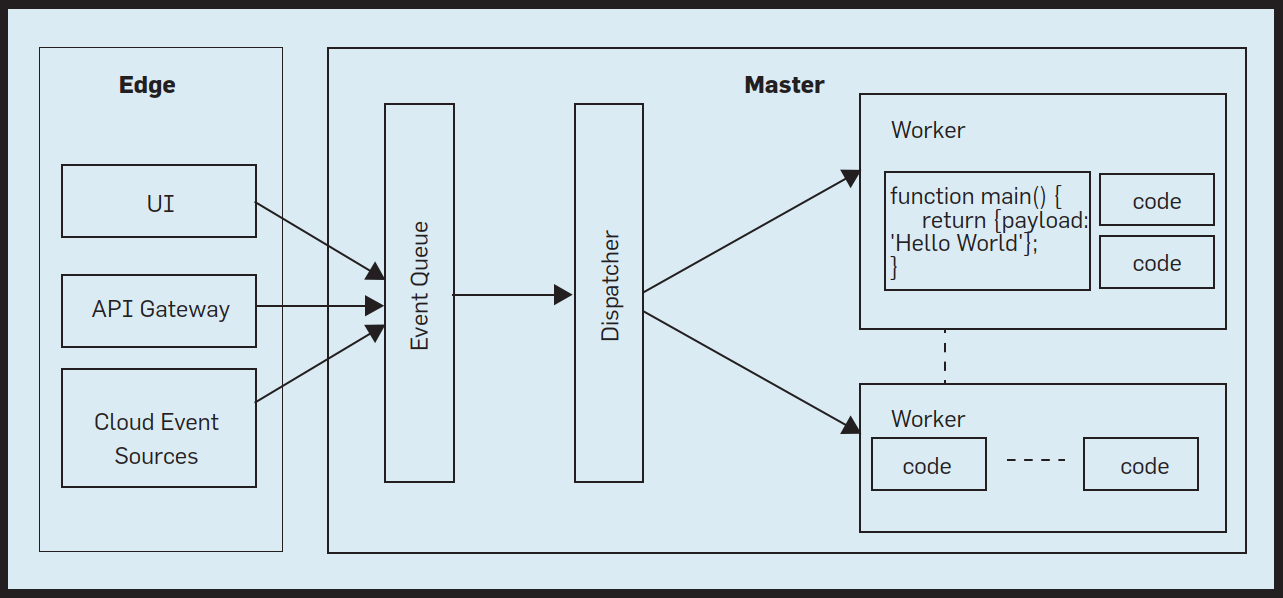
\includegraphics[scale=0.2]{bilder/FaaS_architecture.png}
\captionsetup[table]{justification=centering, labelfont=bf}
\caption{\vs{TO REDO: identify which components are being benchmarked. Serverless FaaS platform architecture}\cite{riseofserverless}\label{fig:faas_arch}}
\end{center}
\end{figure}
%(see figure \ref{fig:iaas}). 
%With most cloud service providers, the user can upload an application (this can be in the form of source code, binaries or even a Docker image) and define a trigger (\gls{HTTP}, Storage, Database, etc.) which invokes the function. 
%This can be useful for application backends and data processing \cite{AWSLambda, GoogleFunctions}. 
%By the help of this technology, users can implement their services without either buying or renting a server or a \gls{VM} in the cloud. 
%They can for example create a backend service without thinking about hardware and server management. 


Despite the convenience of the appraoch, we observe how several open questions remain unsolved. %some issues remain unresolved and some questions stay open. 
Namely, it is currently hard to decide on a specific cloud provider based on criterias such as performance, workload adaptability or costs.
%Which cloud provider to choose to run an application on? Can the cloud provider handle the load? How much is it going to cost? 
This paper introduces \sys, a testing suite that tackles these questions by providing a benchmark and testing suite for serverless computing. 
%With this suite 
A cloud user can use the suite to deploy several tests and observe how different cloud providers perform. % and the suite helps to make the decision easier.

While few efforts exist to benchmark serverless computing~\cite{doi:10.1002/cpe.4792, Kuntsevich:2018:DAB:3284014.3284016, EoPSCE, 10.1007/978-3-319-75178-8_34}, they ...\vs{fill in with 1 sentence saying why those efforts are not sufficient/clear/poor/}. 
Similarly, studies on benchmarking cloud platforms lack an in-depth evaluation of serverless computing platforms~\cite{Gan:2019:OBS:3297858.3304013}. 


\vs{we need to say what are the main contributions of this work}
\vs{then, say how the paper is organized.} 
 
%\subsection{Cloud Computing}
%The \gls{NIST} defines cloud computing as a model which enables ubiquitous, on-demand network access to computing resources which can be rapidly and easily provisioned and released \cite{Mell:2011:SND:2206223}. Computing resources can be servers (dedicated hardware or \gls{VM}s), storage, applications, services, etc. Those resources are managed by a cloud service provider in their data centers and are normally accessible to everyone on a pay per usage model. The \gls{NIST} also states the following \textbf{essential characteristics} of cloud computing \cite{Mell:2011:SND:2206223}.
%\begin{itemize}
%    \item \textbf{On-demand self service:} A user can provision computing resources automatically and by himself.
%    \item \textbf{Broad network access:} The resources are available over network, typically over a website or a \gls{CLI}.
%    \item \textbf{Resource pooling:} Physical and virtual resources are pooled, used in a multi-tenant model and dynamically assigned depending on demand. The user has no control neither knowledge of the specific location where his resources are allocated, only on a higher level e.g. which data center.
%    \item \textbf{Rapid elasticity:} Services and resources can be elastically and mostly automatically provisioned and scale rapidly. To a user, the available resources seem unlimited at any time.
%    \item \textbf{Measured service:} Resource allocation happens automatically and is optimized by gathering metrics about the resources. The usage of resources can be controlled and monitored transparently for both parties and also benefits both.
%\end{itemize}
%
%Besides the essential characteristics there are also three service models and four deployment models which will be described in the following \cite{Mell:2011:SND:2206223, IBMCC}.\\
%\newline
%\textbf{Service models}
%\begin{itemize}
%    \item \textbf{\gls{IaaS}:} The consumer can provision processing (i.e. servers), storage and network components. The user does not control the underlying infrastructure. However, he has control over the operating system, storage and applications. There is also only limited control over the network (i.e. firewalls). A good example would be a \gls{VM} on \gls{AWS} \gls{EC2}.
%    \item \textbf{\gls{PaaS}:} The user can deploy applications on the cloud infrastructure within the provider's supported programming languages, services and tools. He has no control over the \gls{OS} nor the storage, only the application itself, its data and some configuration parameters. An example for \gls{PaaS} is Google App Engine.
%    \item \textbf{\gls{SaaS}:} The consumer uses the provider's applications as they are. The user has no control over the applications capabilities. Usually such software is accessed through a web browser (i.e. website) or other clients. An example of this model is Microsoft Office 365.
%\end{itemize}
%Figure \ref{fig:iaas} shows where the responsibilities are with which service model.
%
%\begin{figure}[htp]
%\begin{center}
%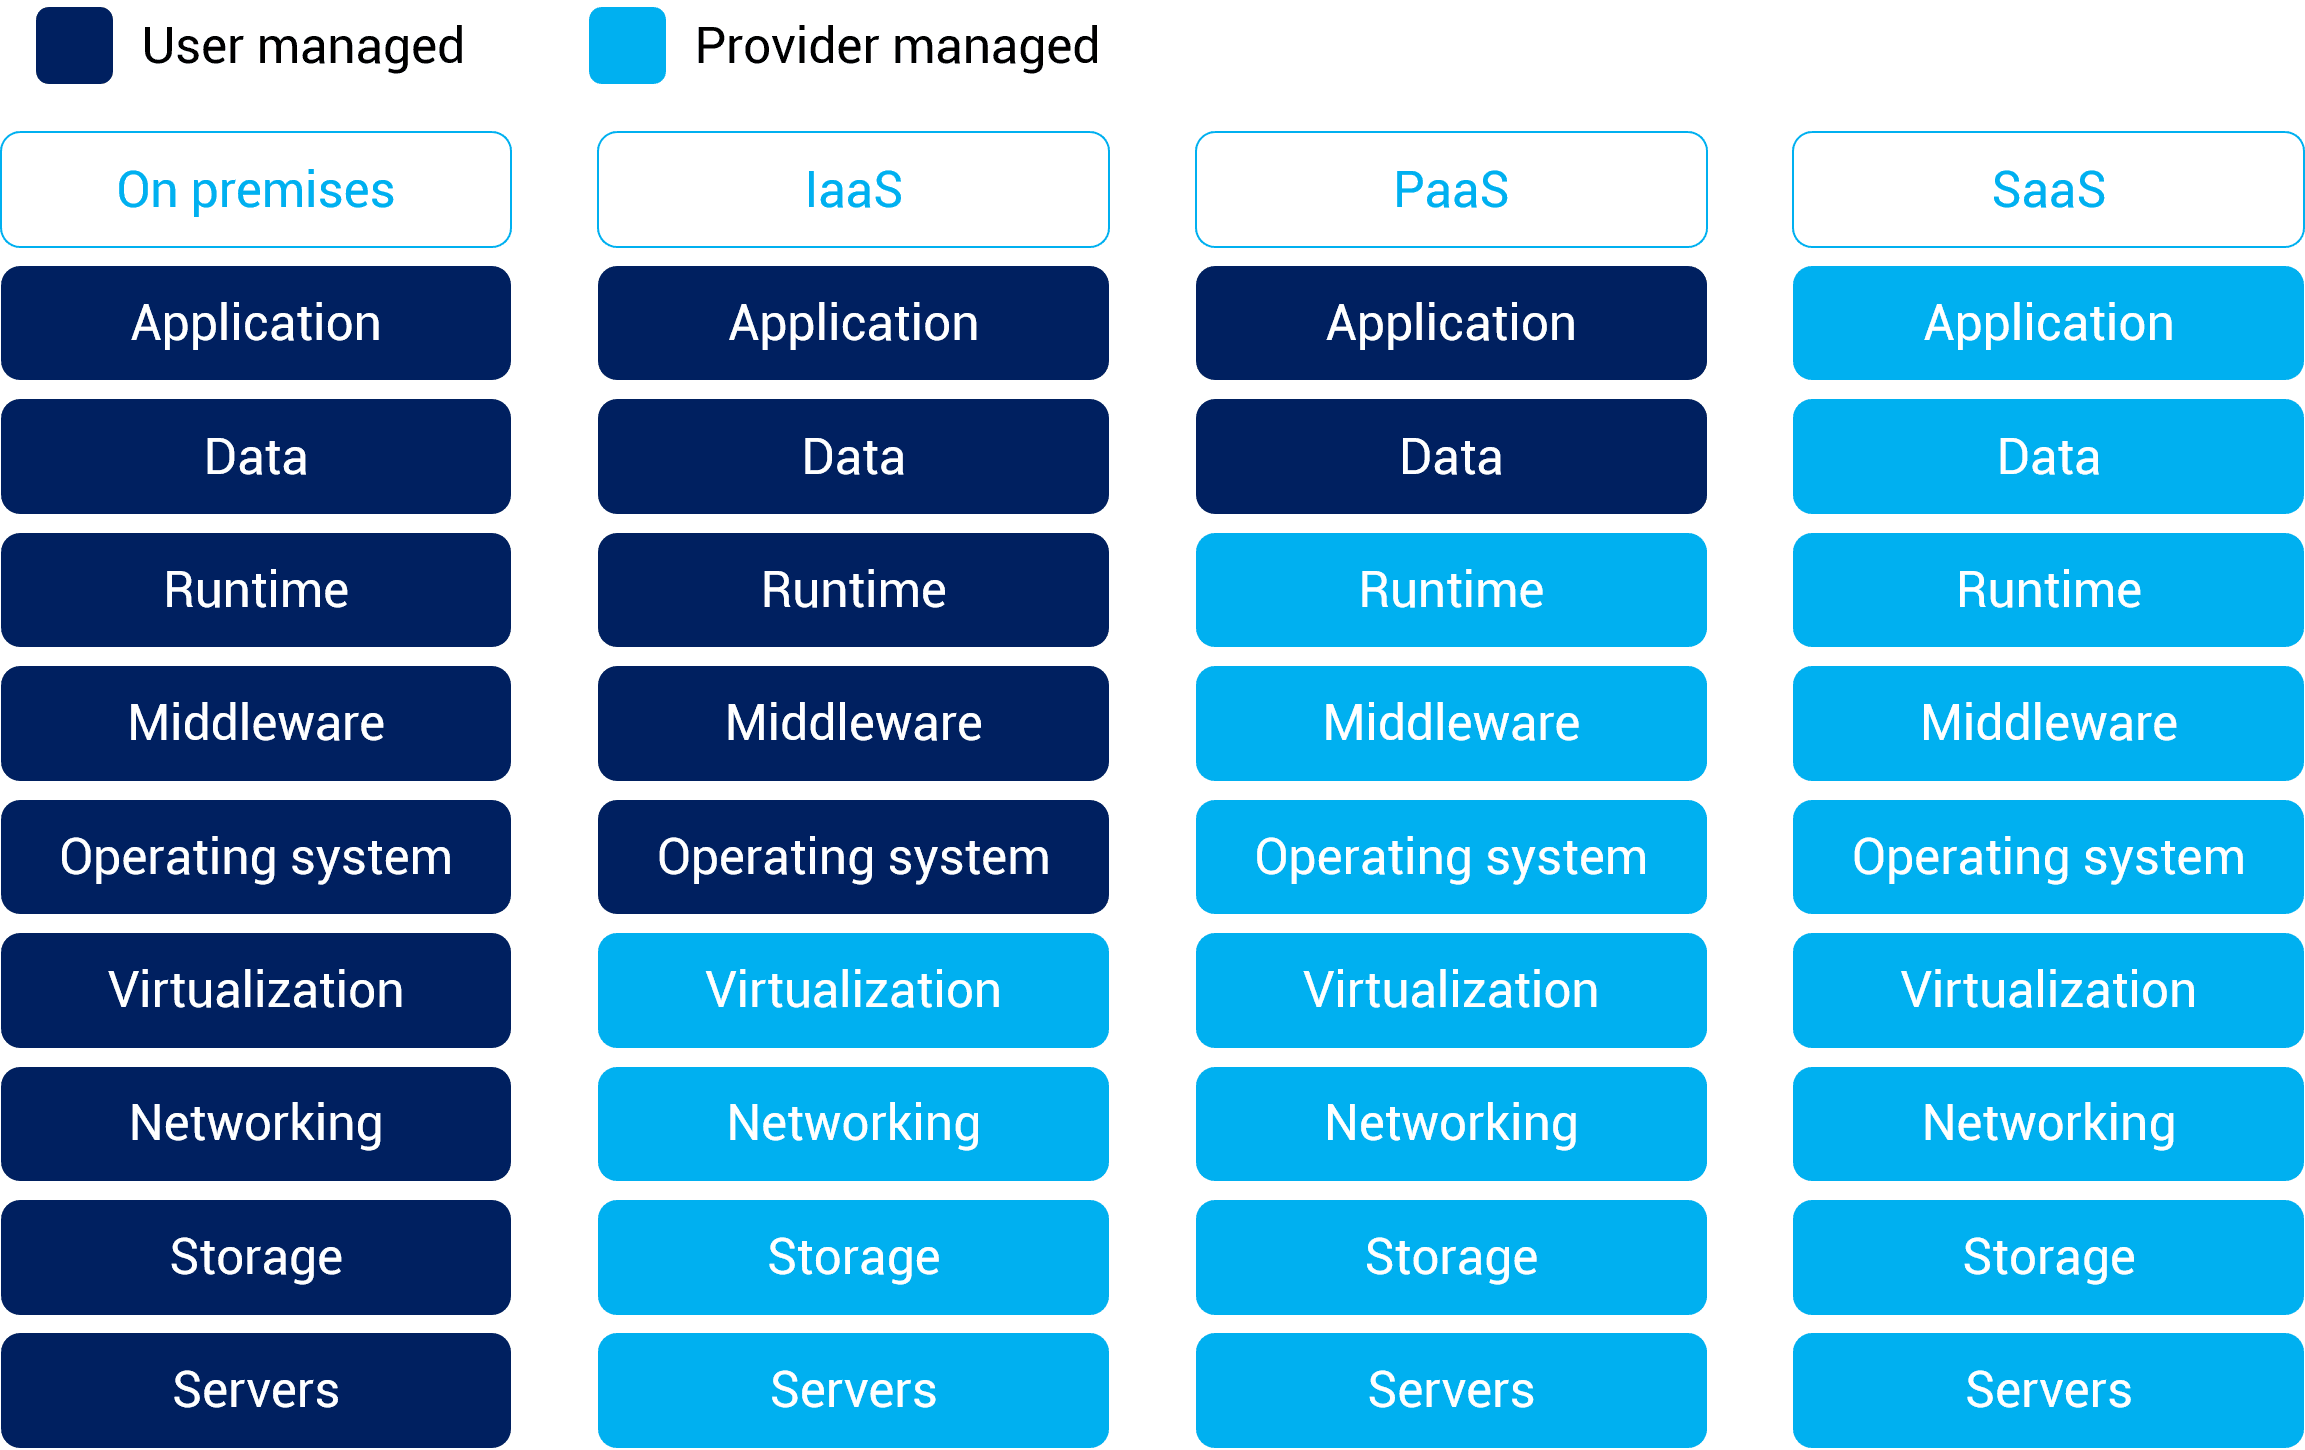
\includegraphics[width=0.5\textwidth]{bilder/iaas.png}
%\captionsetup[table]{justification=centering, labelfont=bf}
%\caption[On premises - IaaS - PaaS - SaaS]{On premises - IaaS - PaaS - SaaS\\Source: Alibaba Cloud \cite{alibaba}}
%\label{fig:iaas}
%\end{center}
%\end{figure}
%
%\textbf{Deployment models} \cite{Mell:2011:SND:2206223}
%\begin{itemize}
%    \item \textbf{Private cloud:} The infrastructure is exclusive to an organization. It can be owned and managed by the organization itself, but also by a third party. The private cloud can exist on or off premise.
%    \item \textbf{Community cloud:} A community cloud is very similar to a private cloud with the difference that it is provided for a specific community with common interests. It can be owned and managed by the community or a third party and can also be on or off premise.
%    \item \textbf{Public cloud:} The infrastructure is generally available to the public. It is typically owned and managed by the organization that runs it and is located on their premises.
%    \item \textbf{Hybrid cloud:} A hybrid cloud is a mixture of the above three types. Each type remains a separate unit, but is interconnected with the other units. In practice, this is often seen with companies who switch to a public cloud. They use a combination of private and public cloud and can therefore migrate application by application to the public cloud until all runs in the public cloud.
%\end{itemize}
%The German Federal Office for Information Security also shares this definition of cloud computing from the \gls{NIST} and has adopted it in principle more or less literally \cite{BSICC}.\\
%This thesis will be only treating public clouds and a slightly different service model called Function as a Service (\gls{FaaS}). It will be explained in the next section \ref{sec:serverless}.

%\textbf{Serverless Computing.}
%As defined by \gls{IBM} in \cite{serverlessibm}, "serverless is an approach to computing that offloads responsibility for common infrastructure management tasks (\emph{e.g.}, scaling, scheduling, patching, provisioning, etc.) to cloud providers and tools, allowing engineers to focus their time and effort on the business logic specific to their applications or process".
%Serverless requires less expertise than other self-managed approaches.
%Infact, users don't manage directly the operating infrastructure, delegating the (automatic) scaling directly to the cloud provider.
%This approach allows the providers to charge only for the given service offered~\cite{serverlessaws, serverlessazure}.

%Using serverless technologies requires much less expertise than non serverless self managed implementations. 
%Although those technologies might come with certain limitations or performance bottlenecks that won't fit to the user's needs.\\
%The most important key features of serverless computing are the following: 
%No server or infrastructure management of the user is required, the workload is scaled dynamically and automatically and it is usually paid per usage, e.g. only charged for the occupied storage in a service \cite{serverlessaws, serverlessazure}.\\
%There exists three main serverless offerings: \emph{(1)} FaaS (Function as a Service, \emph{e.g.}, \gls{AWS} Lambda), \emph{(2)} DBaaS (Database as a Service, \emph{e.g.} Microsoft Azure Database for PostgreSQL) and \emph{(3)} STaaS (Storage as a service, \emph{e.g.}, Google Cloud Storage \cite{serverlessgoogle}). 

%This thesis will treat the domain of FaaS.
%\subsection{FaaS (Function as a Service)}




%\subsection{Benchmarking}
%Benchmarking is a method to analyze and test the performance of a system, to discover its benefits and weaknesses and to compare it directly to other systems. 
%In this thesis, the systems will be serverless platforms and they will be tested with different applications to see how fast they run, how well they scale and how much they cost. 
%In order to get meaningful results, these tests should be executed as similar as possible on each system and repeated enough times to avoid coincidental data. In the following chapters the systems, the tests, the benchmark process and the results will be carefully discussed and explained in detail.


%!TEX root = main.tex
\section{Background}
This section provide technical details about the four main serverless providers, namely Amazon Web Services (\S\ref{sec:ss:aws}), Microsoft Azure (\S\ref{sec:ss:azure}), Google Cloud (\S\ref{sec:ss:google}) and IBM Cloud (\S\ref{sec:ss:ibm}). 
\vs{MAISSEN that the next sentence is true:} We compare the performance of all of them in our evaluation (see Section~\ref{sec:evaluation}).

%In this chapter, the choice of serverless computing providers and the choice of runtimes respectively programming languages is derived. Furthermore, the implemented tests will be explained in detail and it is shown what their effect and importance is.

%\subsection{Choosing Serverless Computing Providers}
%\label{sec:CSP}
%
%There are a lot of cloud providers available and many of them are trying to grow and therefore investing more and more in their infrastructure. So this benchmark suite could have taken into account as many cloud providers as possible, assumed they provide serverless computing, but that would have exceeded the scope of this thesis. Figure \ref{fig:market_share} illustrates on the left hand side the global revenue of the cloud infrastructure services market which has reached nearly \$23 billion in the second quarter of 2019. What's more interesting for choosing cloud providers for this benchmark suite is the market share. As one can see in figure \ref{fig:market_share} on the right hand side the market share of cloud computing is mainly dominated by a few big players: Amazon, Microsoft, Google, \gls{IBM} and Alibaba. Amazon still is the unprecedented leader in this field of business. Nevertheless, other competitors are heavily investing in the cloud business. Google will invest 3 billion euros in its European data centers as Sundar Pichai, the \gls{CEO} of Google, stated in the Google blog \cite{GoogleBlog}. And also Microsoft has recently been given a \$10 billion contract by the US Department of Defense to transform the military's cloud computing systems \cite{NYJEDI, JEDI}.
%
%\begin{figure}[htp]
%\begin{center}
%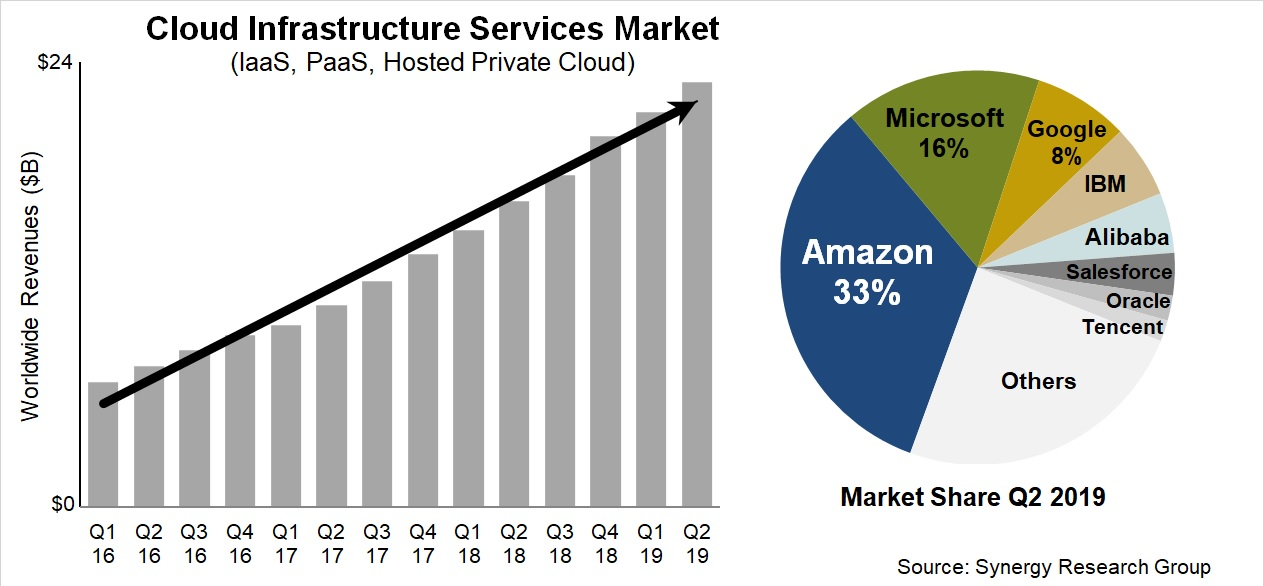
\includegraphics[width=0.5\textwidth]{bilder/synergy.jpg}
%\captionsetup[table]{justification=centering, labelfont=bf}
%\caption[Cloud Infrastructure Services Market Share]{Cloud Infrastructure Services Market Share\\Source: Synergy Research Group \cite{Synergy}}
%\label{fig:market_share}
%\end{center}
%\end{figure}
%
%For the above mentioned reasons, the following top four providers were taken into consideration.
%\begin{itemize}
%  \item Amazon Web Services
%  \item Microsoft Azure
%  \item Google Cloud
%  \item IBM Cloud
%\end{itemize}
%All of them offer a serverless platform which will be described for each cloud provider in the following sections.

%\begin{remark}
%At the beginning of this thesis, a deployment on Apache OpenWhisk was considered on the private cluster of the university of Neuchâtel. After several time wasting and failed attempts to set up OpenWhisk and contradicting documentation on the OpenWhisk website respectively the GitHub page of OpenWhisk the idea was dropped. Since \gls{IBM} uses an implementation based on OpenWhisk, the performance is expected to be similar. Nevertheless, it would have been interesting to compare those two very similar or even identical systems on a private and on a public cloud.
%\end{remark}

\subsection{Amazon Web Services Lambda}\label{sec:ss:aws}

\gls{AWS} Lambda~\cite{AWSLambda} was released in November in 2014 \cite{AWSLambdaRelease}. 
\gls{AWS} Lambda spans 18 geographically dispersed regions, plus China\cite{AWSRegions}. 
At the time of writing, it supports six different runtimes and seven different programming languages \cite{AWSLambdaLanguages}. 
Depending on the region where the function is deployed, Lambda supports up to 3000 instances to serve the user' functions~\cite{AWSLambdaScaling}. 
The memory allocated to a function instance can vary from 128 \gls{MB} up to 3008 \gls{MB} in steps of 64 \gls{MB}~\cite{AWSLambdaConfig}. 
The \gls{CPU} power increases linearly with its memory allocation.
Forinstance, at 1792 \gls{MB} the function will get 1 \gls{vCPU}~\cite{AWSLambdaConfig}.\vs{MAISSEN: why 1792?}

As observed in~\cite{216063}, Lambda executes functions using two different \gls{CPU}s, namely Intel Xeon E5-2666 clocked at 2.90 \gls{GHz}  and the Intel Xeon E5-2680, clocked at 2.80 \gls{GHz} respectively. 
%This information was extracted by Wang et al. from the file \texttt{/proc/cpuinfo} in the Linux operating system.
%\begin{remark} From my own experience I can tell that cloud providers generally don't like to tell their customers every detail of hardware they use or how exactly services are implemented. The first point might be true because they don't want to tell a customer what exact \gls{CPU}s he gets, because then he will certainly complain if it differs from the specification and the provider has to take responsibility. The second point should be obvious for economic and competition related reasons.
%\end{remark}
%Knowing that, one can more or less estimate the theoretical computing power that the virtual \gls{CPU} will provide. 
%\begin{remark}
%The pricing of \gls{AWS} Lambda and all the other services will be discussed in section \ref{sec:pricing} Pricing.
%\end{remark}

\subsection{Microsoft Azure Functions}\label{sec:ss:azure}

Microsoft Azure Functions~\cite{AzureFunctions} was released publicly in Novenber 2016~\cite{AzureFunctionsAnnouncement}. %in preview (Microsoft's term for beta) and then later in November 2016 it became generally available \cite{AzureFunctionsAnnouncement}. 
it supports five runtimes and seven different programming languages~\cite{AzureFunctionsLanguages}.
Compared to the other three cloud providers, Azure offers three different hosting plans \cite{AzureFunctionsPlans}:
%Something a little different with Azure compared to the other three cloud providers is that one can select between three different hosting plans \cite{AzureFunctionsPlans}:
Azure Functions offers billing plans that adapt to the load and popularity of the deployed function (\emph{e.g.}, the consumption plan), plans with finer-grain control over the computing instance size and pre-warming support (\emph{e.g.}, a premium plan), and an billing plan customized on a given application needs (\emph{e.g.}, the app service plan). 
This work only considers the consumption plan (generation 2.0~\cite{AzureFunctionsGenerations}), being the only one to be fully managed by the cloud provider and the most similar in the features to the ones offered by the alternative provders. 
%\begin{itemize}
%\item[] \textbf{Consumption plan:} It adds and removes instances dynamically depending on the load on the function and cost only arise when functions are running. This is the most 'serverless' option among those three.
%\item[] \textbf{Premium plan:} The premium plan is similar to the consumption plan but offers more integration and control over the functions. Instance sizes can be chosen and instances can be pre-warmed. The cost is calculated with \gls{CPU} and \gls{GB} memory used per second.
%\item[] \textbf{App Service plan:} How many and on which \gls{VM}s the functions run can be decided in the App Service plan. Scaling happens manually, time based or based on metrics such as \gls{CPU} usage.
%\end{itemize}
%This thesis will only consider the consumption plan, as it is the default plan and fully managed, and therefore \textit{more} serverless than the others. Additionally, it is similar to the services of the other providers.\\
%There are currently three different generations of the service available \cite{AzureFunctionsGenerations}, this project uses generation 2.

Azure Functions can use as many as 200 instances and up to 1.5GB memory~\cite{AzureFunctionsPlans}. 
The service can run either on Windows or Linux hosts, and is offered in 28 out of 46 publicly accessible regions~\cite{AzureRegions}.
Note that the consumption plan is only available in 11 regions for both Linux and Windows, hence we restrict to those in our experiments.
Computing nodes can be characterized by their \gls{ACU}, with 100 ACU roughly map to 1 \gls{vCPU}.
%For computing power, Azure has its own term named \gls{ACU} index, where 100 ACU roughly map to 1 \gls{vCPU}.
%The instances in the Azure functions consumption plan have an \gls{ACU} of 100 which is about the equivalent of 1 \gls{vCPU}. 
According to our investigations, we believe Azure Functions to be executed by virtual machiens of type \textit{Av2}\vs{MAISSEN: which ones from \url{https://aws.amazon.com/ec2/instance-types/}? Clarify.}, as it most closely resembles its declared \gls{ACU}~\cite{AzureFunctionsVMs}. 
These \gls{VM}s use three different \gls{CPU}s: Intel Xeon 8171M at 2.1 \gls{GHz}, Intel Xeon E5-2673 v4 at 2.3 \gls{GHz} and Intel Xeon E5-2673 v3 at 2.4 \gls{GHz}~\cite{AzureFunctionsVMs}.

\subsection{Google Cloud Functions}\label{sec:ss:google}
%\vs{STOPPED HERE}
%On the Google Cloud Platform, the serverless service is simply called \textit{Functions} \cite{GoogleFunctions}. 
Google Functions~\cite{GoogleFunctions} was released on July in 2018~\cite{GoogleFunctionsReleases}, and currently available through seven out of twenty regions~\cite{GoogleFunctionsLocations}.
%Compared to AWS and Azure that is two and a half years respectively one year later for the first release. 
It currently only supports three programming languages~\cite{GoogleFunctionsLanguages}, namely \vs{MAISSEN: FIX}. 
While there is not a maximum number of allocated instances per single function, it only allows up to 1000 functions to be executed concurrently~\cite{GoogleFunctionsQuotas}.
%The documentation does not mention a limit of maximum allocated instances per function. 
%However, it states that at maximum 1000 functions can be concurrently in execution \cite{GoogleFunctionsQuotas}.
Table~\ref{table:google_functions_cpu_ram} summarizes the options for CPU and memory combinations supported by the platform\cite{GoogleFunctionsPricing}.
While the official \emph{Functions} documentation lacks details on the exact CPU models, a quick inspection of \texttt{/proc/cpuinfo} unveils certain details, such as \texttt{vendor\_id}, \texttt{cpu\_family} and \texttt{model}.
We report on the use of Intel-based processors as well as some specific generation details in \vs{MAISSEN: FIX where?}.
%Possible options for CPU and memory allocation per instance are shown in table \ref{table:google_functions_cpu_ram} \cite{GoogleFunctionsPricing}. 
%The service is available in seven out of twenty regions~\cite{GoogleFunctionsLocations}.

\begin{table}[!t]

\caption[Google Cloud Functions - Possible memory allocation and corresponding CPU frequency]{Google Cloud Functions - Possible memory allocation and corresponding CPU frequency~\cite{GoogleFunctionsPricing}.}
%\captionsetup[table]{justification=centering, labelfont=bf}
\centering
\resizebox{\columnwidth}{!}{
\begin{tabular}{l|r|r|r|r|r} 
 \hline
	\textbf{Memory} & 128\gls{MB} & 256\gls{MB} & 512\gls{MB} & 1024\gls{MB} & 2048\gls{MB} \\ 
	\textbf{CPU} & 200\gls{MHz} & 400\gls{MHz} & 800\gls{MHz} & 1.4 \gls{GHz} & 2.4 \gls{GHz} \\
	\hline
\end{tabular}
\vspace{-10pt}
}
\label{table:google_functions_cpu_ram}
\end{table}

%Google does not mention what type of CPU they use for functions on the underlying infrastructure. 
%The CPU type could also not be extracted by Wang et al. \cite{216063} and the file \texttt{/proc/cpuinfo} does not show information on the CPU model name. 
%It shows however information for the fields \texttt{vendor\_id}, \texttt{cpu\_family} and \texttt{model}. 
%Those values reveal that Intel processors are used and can give an indication from which generation the CPU is. 
%\vs{See the example file content \ref{lst:cpuinfo} in the appendix.} 

\subsection{IBM Cloud Functions}\label{sec:ss:ibm}

\gls{IBM}'s Cloud Functions \cite{IBMFunctions} is built atop Apache OpenWhisk, an open source serverless cloud platform using Docker containers~\cite{OpenWhisk}. 
As such, in addition to Docker, it supports eight additional runtimes~\cite{IBMRuntimes}, such as \vs{MAISSEN: list them all here}.
%\gls{IBM} Cloud Functions supports nine different runtimes including a Docker runtime \cite{IBMRuntimes}. 
The service is restricted to 1000 concurrently active executions (including those enqueued for execution) per namespace~\cite{IBMLimits}. 
%However this limit can be increased for a specific business case but needs to be applied for via the ticketing system of the \gls{IBM} support \cite{IBMLimits}. 
Memory allocation can be set from 128 \gls{MB} to 2048 \gls{MB} in steps of 32 \gls{MB}. 
\gls{IBM} Cloud Functions is available in five out of six regions \cite{IBMLocations}.\footnote{One region\vs{MAISSEN: which one?} lacks support for Cloud Foundry~\cite{IBMCloudFoundry} and as such it not be used to deply via the \gls{CLI}, and hence it is not included in this work.} 
%The documentation does not mention anything on \gls{CPU} or machines they are using. 
Our experiments revelaed that some of the  instances supporting the execution of the functions run on top of Intel Xeon E5-2683 v3 at 2.00 \gls{GHz}.
\vs{See the example file content \ref{lst:cpuinfo2} in the appendix.}




%!TEX root = main.tex
\section{Choosing Runtimes}\label{sec:runtime}
This section dscribes the supported runtimes and respective programming languages supported by the serverless providers described in \ref{sec:background}. 
%After the technical description and specification of each provider, the following section will deduct which runtimes respectively programming languages were chosen and why.\\
Table~\ref{table:programming_languages} shows our survey. %all supported runtimes for each cloud service provider mentioned in section \ref{sec:background}. 
\vs{MAISSEN: remove this column, not needed in the large table we discussed via email --- On the right hand side there is the sum for each runtime, which indicates the number of cloud service providers supporting that runtime.}

\begin{table}[!t]
\centering
\captionsetup[table]{justification=centering, labelfont=bf}
\resizebox{\columnwidth}{!}{
\begin{tabular}{l|c|c|c|c|c||l} 
% \hline
 & \multirow{2}{*}{AWS} & \multicolumn{2}{c|}{Azure} & \multirow{2}{*}{Google} & \multirow{2}{*}{IBM} & \multirow{2}{*}{Sum} \\ \cline{3-4}
  & & Linux & Windows & & & \\ \hline
  Node.js &  \cellcolor{green!25}yes & \cellcolor{green!25}yes & \cellcolor{green!25}yes & \cellcolor{green!25}yes & \cellcolor{green!25}yes & 4.0 \\ \hline
  Python & \cellcolor{green!25}yes & \cellcolor{green!25}yes & \cellcolor{red!25}no & \cellcolor{green!25}yes & \cellcolor{green!25}yes & 3.5 \\ \hline
  .NET Core & \cellcolor{green!25}yes & \cellcolor{green!25}yes & \cellcolor{green!25}yes & \cellcolor{red!25}no & \cellcolor{green!25}yes & 3.0 \\ \hline
  Go & \cellcolor{green!25}yes & \cellcolor{red!25}no & \cellcolor{red!25}no & \cellcolor{green!25}yes & \cellcolor{green!25}yes & 3.0 \\ \hline
  Java & \cellcolor{green!25}yes & \cellcolor{red!25}no & \cellcolor{green!25}yes & \cellcolor{red!25}no & \cellcolor{green!25}yes & 2.5 \\ \hline
  Ruby & \cellcolor{green!25}yes & \cellcolor{red!25}no & \cellcolor{red!25}no & \cellcolor{red!25}no & \cellcolor{green!25}yes & 2.0 \\ \hline
%  PowerShell & \cellcolor{green!25}yes & \cellcolor{red!25}no & \cellcolor{green!25}yes & \cellcolor{red!25}no & \cellcolor{red!25}no & 1.5 \\ \hline
  Swift & \cellcolor{red!25}no & \cellcolor{red!25}no & \cellcolor{red!25}no & \cellcolor{red!25}no & \cellcolor{green!25}yes & 1.0 \\ \hline
  PHP & \cellcolor{red!25}no & \cellcolor{red!25}no & \cellcolor{red!25}no & \cellcolor{red!25}no & \cellcolor{green!25}yes & 1.0 \\ \hline
  Docker & \cellcolor{yellow!25}ECS & \cellcolor{green!25}yes & \cellcolor{red!25}no & \cellcolor{yellow!25}Cloud Run & \cellcolor{green!25}yes & 1.5 \\
 \hline
\end{tabular}
}
\caption[Supported runtimes in serverless computing]{Supported runtimes in serverless computing.  Data source: \cite{AWSLambdaLanguages, AzureFunctionsLanguages, GoogleFunctionsLanguages, IBMRuntimes}. \vs{MAISSEN: If the yellow color does not mean the same thing in as in the nodejs table, use  markers/symbols next to the value of the cell to identify specific conditions/exceptions.}}
\label{table:programming_languages}
\end{table}

For the sake of comparisons and fairness of benchmarking, we are interested in runtimes and programming languages supported by multiple cloud providers.  
Table~\ref{table:programming_languages} highlights the following facts.
First, we observe that Node.js\vs{REF} is supported by all clouds \vs{MAISSEN: why is that? is it because it is a cloud-native language? just very popular?}. 
Python is similarly well supported, except by Azure with Windows \gls{OS}\vs{MAISSEN: from \ref{table:python}, this seems not to be totally true}.
Microsoft's \texttt{.NET Core} lacks support from Google \vs{MAISSEN: add missing details, we cannot say$\rightarrow$ and so forth}. 
In the reminder of this paper, including our evaluation of \sys, we focus our comparison on the top best supported runtimes, namely \vs{MAISSEN: say which ones}. 
%A brief summary of each runtime will be given in the following subsections.

\begin{remark}	
\vs{Maybe we can move this remark in the previous section where we describe the providers ?}
Azure has currently three different generations of its service\vs{MAISSEN: add url}. 
The first generation is currently in maintenance, while the two other ones remain available. 
The available runtimes in the next section will only consider generation 2 (which is also used in this project):
\end{remark}

\textbf{Node.js.} Node.js is a JavaScript runtime built on Chrome's V8 JavaScript engine~\cite{Nodejs}. 
%As the name indicates, JavaScript is a scripting language and was first released on the 4th December 1995 by Netscape \cite{JavaScript}. 
%It was mostly used in addition to \gls{HTML} and \gls{CSS} in web browsers \cite{JavaScript}. 
Because of the Node.js framework and the \gls{NPM}, JavaScript is nowadays a popular language to implement all kinds of applications\vs{MAISSEN: it'd be good to add a link, for instance to the tiobe popularity index \url{https://www.tiobe.com/tiobe-index/}}. 
Table \ref{table:nodejs} shows supported Node.js versions of each cloud provider. 

\begin{table}[!t]
\centering
\captionsetup[table]{justification=centering, labelfont=bf}
\begin{tabular}{l|c|c|c|c} 
% \hline
 Node.js & AWS & Azure & Google & IBM \\ \hline
6.x  & \cellcolor{red!25}no    & \cellcolor{red!25}no    & \cellcolor{yellow!25}yes  & \cellcolor{red!25}no\\ \hline
8.x  & \cellcolor{red!25}no & \cellcolor{green!25}yes & \cellcolor{green!25}yes   & \cellcolor{green!25}yes \\ \hline
10.x & \cellcolor{green!25}yes & \cellcolor{green!25}yes & \cellcolor{yellow!25}yes  & \cellcolor{green!25}yes \\ \hline
12.x & \cellcolor{green!25}yes & \cellcolor{red!25}no & \cellcolor{red!25}no & \cellcolor{red!25}no \\ \hline
\end{tabular}
\caption[Supported Node.js runtimes]{Supported Node.js runtimes~\cite{AWSLambdaLanguages, AzureFunctionsLanguages, GoogleFunctionsLanguages, IBMRuntimes}\\. Yellow=\textit{deprecated} and \textit{beta} for version 6.x and 10.x.}
\label{table:nodejs}
\end{table}

Due to its vast support from all providers, \sys will deploy all Node.js applications using version 10.x. 
%In particular, \gls{AWS} uses version 10.x \cite{AWSLambdaLanguages}, Azure does not specify more than version 10 \cite{AzureFunctionsLanguages}, Google uses version 10.15.3 \cite{GoogleFunctionsRuntimes} and \gls{IBM} implements version 10.15.0 \cite{IBMRuntimes}.

%\begin{remark}
%Google has Node.js version 10 still in beta while Node.js version 8 End-of-life was on December 31, 2019 \cite{NodejsReleases}.
%\end{remark}

\textbf{Python.}
%Python is a universal, open-source and very popular programming language. It was released in 1991 and created by Guido van Rossum \cite{PythonIntro} and runs basically anywhere \cite{PythonAbout}. Python was designed to be very easy to learn and to have readable code \cite{PythonIntro}. It only uses indentation and whitespaces to define the scope of loops, functions and classes \cite{PythonIntro}. Because of those characteristics, developers can implement new features very fast. Cuong Do, software architect of YouTube, said: "Python is fast enough for our site and allows us to produce maintainable features in record times, with a minimum of developers." \cite{PythonQuotes}. 

Table~\ref{table:python} shows the support offered by the various cloud providers to the Python runtime. % which of the four cloud provider supports which Python versions.
At the time of this writing, all cloud providers support version 3.7, hence we rely on this version for our benchmarking results.

\begin{table}[!t]
\centering
\captionsetup[table]{justification=centering, labelfont=bf}
\begin{tabular}{l|c|c|c|c} 
% \hline
 Python & AWS & Azure & Google & IBM \\ \hline
2.7  & \cellcolor{green!25}yes    & \cellcolor{red!25}no    & \cellcolor{red!25}no  & \cellcolor{green!25}yes\\ \hline
3.6  & \cellcolor{green!25}yes & \cellcolor{green!25}yes & \cellcolor{red!25}no   & \cellcolor{green!25}yes \\ \hline
3.7 & \cellcolor{green!25}yes & \cellcolor{green!25}yes & \cellcolor{green!25}yes  & \cellcolor{green!25}yes \\ \hline
3.8 & \cellcolor{green!25}yes & \cellcolor{red!25}no & \cellcolor{red!25}no  & \cellcolor{red!25}no  \\ \hline
\end{tabular}
\caption[Supported Python runtimes]{Supported Python runtimes~\cite{AWSLambdaLanguages, AzureFunctionsLanguages, GoogleFunctionsLanguages, IBMRuntimes}}
\label{table:python}
\end{table}


\textbf{Go.}
Go\cite{GoProject} is a procedural open source programming language developed by a team at Google and other contributors \cite{GoDoc, GoProject}. 
%It is a relatively new language and was first released in March 2012 \cite{GoProject}. 
%It is compiled and therefore more efficient than interpreted languages and it has good concurrency mechanisms to benefit from today's multi-core architecture \cite{GoDoc}. 
%Go also has a garbage collector in contrast to C \cite{GoDoc}. 
%On the Go website the following statement can be found: "It's a fast, statically typed, compiled language that feels like a dynamically typed, interpreted language." \cite{GoDoc}. 
%Today, Go is a popular language given that is is easy to learn and write like Python but also very efficient like C. 
Table~\ref{table:go} shows the supported Go versions.

\begin{table}[!t]
\centering
\captionsetup[table]{justification=centering, labelfont=bf}
\begin{tabular}{l|c|c|c|c} 
% \hline
 Go & AWS & Azure & Google & IBM \\ \hline
1.11  & \cellcolor{green!25}yes    & \cellcolor{red!25}no    & \cellcolor{green!25}yes  & \cellcolor{green!25}yes\\ \hline
\end{tabular}
\caption[Supported Go runtimes]{Supported Go runtimes~\cite{AWSLambdaLanguages, AzureFunctionsLanguages, GoogleFunctionsLanguages, IBMRuntimes}. AWS supports all versions of Go 1.x, depending on the version the binary was compiled with and deployed to Lambda.}
\label{table:go}
\end{table}

\vs{MAISSEN: move into the evaluation setup section:} This thesis will use Go 1.11 for its benchmark functions.
\textbf{.NET Core}
%.NET Core is a free and open-source software framework developed by Microsoft and its community \cite{.NETCore}. The first version was released in June 2016 \cite{.NETCoreReleases}. It supports as languages C\texttt{\#}, F\texttt{\#} and Visual Basic \cite{.NETAbout} and is currently on version 3.1 which was released in December 2019 \cite{.NETCoreBlog}. 
%Microsoft has declared its love for Linux when Satya Nadella in the end of 2014 at a Microsoft Cloud Briefing in San Francisco presented a slide which stated "Microsoft  Linux". 
%\cite{MicrosoftCloudBlog}. 
%Since then the company has embraced Linux, open-source software and cross-platform support. 
Table~\ref{table:dotnet} shows the supported .NET Core versions.
Because there is no common supported version, this project will use 2.1 on \gls{AWS} and 2.2 on Azure and \gls{IBM}, but the test functions are implemented is C\texttt{\#}.

\begin{table}[!t]
\centering
\captionsetup[table]{justification=centering, labelfont=bf}
\begin{tabular}{l|c|c|c|c} 
% \hline
 .NET Core & AWS & Azure & Google & IBM \\ \hline
2.1  & \cellcolor{green!25}yes    & \cellcolor{red!25}no    & \cellcolor{red!25}no  & \cellcolor{red!25}no\\ \hline
2.2  & \cellcolor{red!25}no    & \cellcolor{green!25}yes    & \cellcolor{red!25}no  & \cellcolor{green!25}yes\\ \hline
3.1  & \cellcolor{red!25}no    & \cellcolor{red!25}no    & \cellcolor{red!25}no  & \cellcolor{red!25}no\\ \hline
\end{tabular}
\caption[Supported .NET Core runtimes]{Supported .NET Core runtimes~\cite{AWSLambdaLanguages, AzureFunctionsLanguages, GoogleFunctionsLanguages, IBMRuntimes}}
\label{table:dotnet}
\end{table}


%!TEX root = main.tex
\section{Architecture}
\label{sec:architecture}

This section describes the architecture of the \sys prototype, depicted in \autoref{fig:architecture}, as well as providing some additional implementation details (\S\ref{ssec:impl}).
%In this chapter, the implementation of the main application, whose main role is to  orchestrate the execution of the various benchmarks across the cloud providers. 
%We provdie an overview of the varius compoentns and functionalities the components and their functions will be briefly explained and later every main task the user can do will be explained in detail.
%\subsection{Overview}
The architecture includes the supported clouds and the corresponding serverless services (left), the involved Docker images (middle) and their interface with the system (right).
We detail each component next. 

\begin{figure}[!t]
\begin{center}
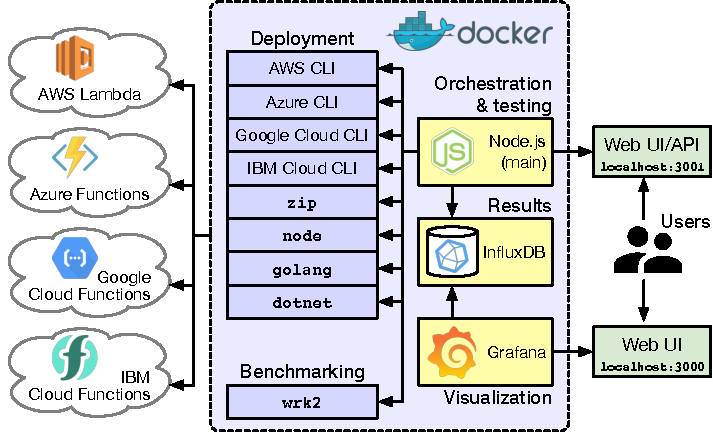
\includegraphics[scale=0.7]{bilder/archi}
\caption{\sys architecture.}
\label{fig:architecture}
\end{center}
\end{figure}

\textbf{Main application.}
The \sys core component is implemented in JavaScript and leverages the Node.js framework. 
It manages all user input and executes the actions or delegates them to other components. 
This application is packaged and executed as Docker containers. 
%Only the Linux packages \texttt{docker-ce} and \texttt{docker-compose} are needed to execute this program. 
%Figure \ref{fig:architecture} depicts all components and gives an overview of the \sys suite.
It manages the following main tasks:
\emph{(1)}~deployment to the clouds;
\emph{(2)}~execution of tests benchmarks; and
\emph{(3)}~computing price estimations. 
Users access it through a Web-based \gls{GUI} or via a REST \gls{API}. 
Once started, the set of configured tests are deployed for execution (some examples are given in \S\ref{sec:tests}).
%After the tests are deployed, they can be tested and benchmarked. 

\textbf{Time series DB.}
\sys uses a time series database (\gls{TSDB}) to store all the results from tests.
These results are subsequently used by graphical interfaces and pricing calculation.
Our prototype uses the InfluxDB~\cite{influx} \gls{TSDB}.

\textbf{UI.}
The \sys architecture provides an API to easily integrate visualization tools.
Our prototype integrates with Grafana~\cite{grafana}, an open source tool to display, plot and monitor data stored in a database. 
The results gathered by the tests and stored in InfluxDB are then displayed in Grafana.

\textbf{CLIs.}
With the exception of AWS, all cloud providers offer a Docker image for their \gls{CLI}. 
Resources can be deployed, deleted and managed completely by the \gls{CLI}.

\textbf{Runtime and languages (Node.js, Go, .NET).}
In addition to the source code of the function(s) to execute, a pre-built and packaged zip file is commonly required to successfully complete the deployment. 
The \sys architecture allows developers to ship runtime images, necessary for instance to install packages and build/run the corresponding code.

%\vs{to remove:
%\textbf{zip:} this image zips the files that need to be deployed to the clouds. 
%Therefore there is no need to have zip installed on the machine the benchmark suite runs.
%}

\textbf{Workload Injectors}.
The \sys architecture provides hook points for plugin workload injectors.
The evaluation results shown in \S\ref{sec:evaluation} uses \texttt{wrk2}~\cite{wrk2}, a stress tool for REST services, to issue requests toward services and gather throughput/latency results.

%%%MOVE TO GITHUB/README
%%%\subsection{Requirements}
%%%\vs{I would move this section completely and have these details in the github/readme page}
%%%To use this application, there are some prerequisite steps necessary. 
%%%First of all, the user needs to have or create accounts on the clouds he intends to test on. 
%%%%This process will be not described in detail since it is straightforward to do. 
%%%%There is however a small guidance for each cloud provider in the documentation on GitHub.\\
%%%Secondly, the user needs to have a Docker environment installed. 
%%%%This is not too difficult on Linux and described exemplary for Ubuntu 18.04 on GitHub.\\
%%%After these steps have been completed some more manual initialization and configuration steps are required from the user. 
%%%He needs to create a few Docker volumes and perform the login process for each \gls{CLI} belonging to the cloud intended to be tested.\\
%%%As last point some free storage is required because some Docker images are quite large, in total around 5.15 GB. 
%%%In addition, some free space should be reserved for the data that will be stored in the database, 1 GB should be sufficient. Table \ref{table:images} shows all images and their sizes.
%%%\begin{table}[htp]
%%%\centering
%%%\captionsetup[table]{justification=centering, labelfont=bf}
%%%\begin{tabular}{|l|l|r|}\hline
%%%\textbf{Repository} & \textbf{Tag} & \textbf{Size} \\ \hline
%%%bschitter/benchmark-suite-serverless-computing	&	0.1	&	358MB	\\ \hline
%%%mikesir87/aws-cli	&	1.16.310	&	186MB	\\ \hline
%%%google/cloud-sdk	&	274.0.1-alpine	&	287MB	\\ \hline
%%%mcr.microsoft.com/azure-cli	&	2.0.78	&	1.04GB	\\ \hline
%%%mcr.microsoft.com/dotnet/core/sdk	&	2.2-alpine3.9	&	1.48GB	\\ \hline
%%%bschitter/alpine-with-zip	&	0.1	&	6.32MB	\\ \hline
%%%bschitter/alpine-with-wrk2	&	0.1	&	232MB	\\ \hline
%%%ibmcom/ibm-cloud-developer-tools-amd64	&	0.20.0	&	309MB	\\ \hline
%%%golang	&	1.11-stretch	&	757MB	\\ \hline
%%%node	&	10.16.2-alpine	&	76.4MB	\\ \hline
%%%grafana/grafana	&	6.3.2	&	254MB	\\ \hline
%%%influxdb	&	1.7.7-alpine	&	137MB	\\ \hline
%%%\textbf{Total size} & & \textbf{5.15GB}\\ \hline
%%%\end{tabular}
%%%\caption[Docker images]{Docker images}
%%%\label{table:images}
%%%\end{table}

\begin{figure}[!t]
\begin{center}
\fboxrule=0.25pt\fbox{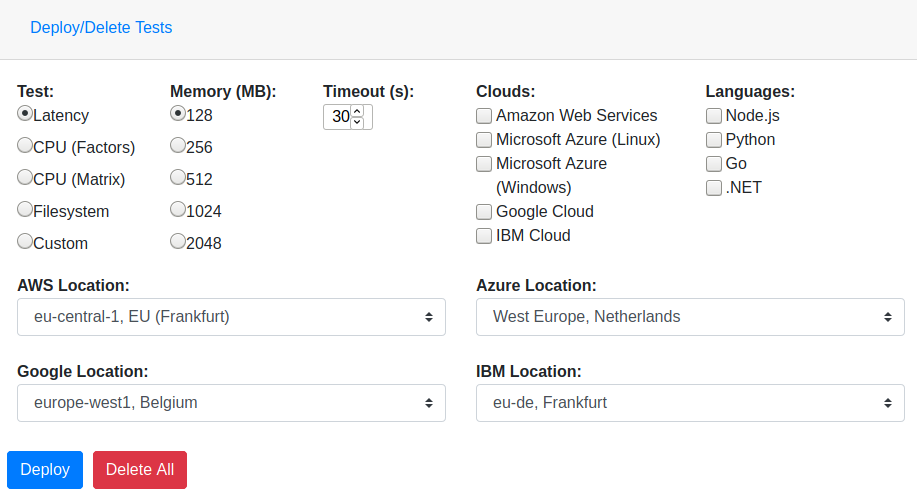
\includegraphics[scale=0.25]{bilder/ui.png}}
\caption{\sys Web-based GUI.}
\label{fig:ui}
\end{center}
\end{figure}

\begin{figure}[!b]
\begin{center}
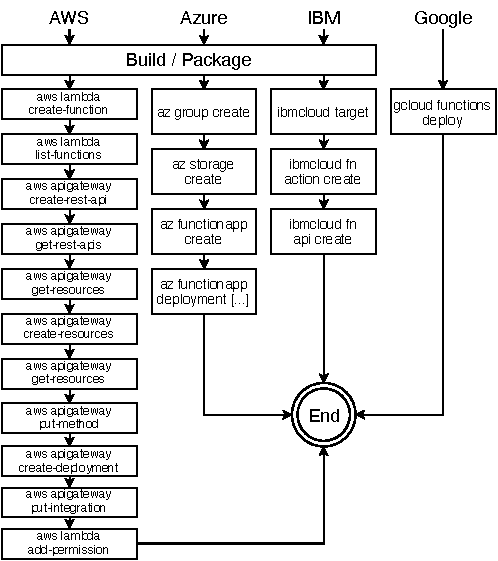
\includegraphics[scale=0.7]{bilder/deploy_flowcharts_small}
\caption{Deployment steps for the different cloud providers supported by \sys.}
\label{fig:flowchart}
\end{center}
\end{figure}

\subsection{Deployment}

%This section will describe the deployment process of the tests.
Once the main application has started, the client can deploy the desired tests, for instance via the Web-based interface shown in \autoref{fig:ui}.
Functions can be parametrized with memory allocated for each instance, timeouts, list of providers and runtime versions to use for the benchmarks, as well as geographical regions (as supported by the cloud provider) where to deploy the tests. 
%\begin{itemize}
%    \item \textbf{Test:} a unique identifier for the test to execute to deploy;
%    \item \textbf{Memory:} The amount of memory to allocate per function.\footnote{Azure assignmes memory dynamically, up to 1536 \gls{MB} per function}
%    \item \textbf{Timeout:} The time limit after which a running function will time out. %\\ \textbf{Remark:} Not applicable for Azure since it handles timeout configuration in a configuration file.
%    \item \textbf{Clouds:} The cloud providers the tests will be deployed on, multiple choices possible.
%    \item \textbf{Languages:} Runtimes respectively languages to deploy the function in, multiple choices possible.
%    \item \textbf{Locations:} The region where the function will be deployed to.
%\end{itemize}
Once deployed, the interface continuously reports on the progress and potential issues (\eg, timeouts, access problems, \etc). 
%Next the \textit{Deploy} button can be pressed and the application will initiate the deployment. On the right hand side of the web interface there will be information about the progress. 
The deployment process is parallelized, including the creation of the required cloud resources, the build and packaging of the functions, and their upload over the cloud.
The deployment flow is slightly different for each provider, with some providers requiring significantly more operations than others.
\autoref{fig:flowchart} illustrates the various steps involved in the deployment for the providers supported by \sys.

Upon cleanup, all deployed functions are permanently deleted, as well as all the configurations and resource groups created at deployment time.

\subsection{Testing}

%In this section it is briefly explained how to execute a test and see its results. 
When testing a serverless execution, \sys will send every five seconds a request to the functions previously deployed, with the purpose to gather baseline results under low, constant load. %As options, a name for the test and the functions parameter can be set. 
\autoref{fig:grafana} illustrates a screenshot of Grafana displaying the results of a latency test in Node.js. 
%At the top, there are three drop down menus to choose the test type, the test name (given at the start of the test) and the data points interval.

\begin{figure}[!t]
\begin{center}
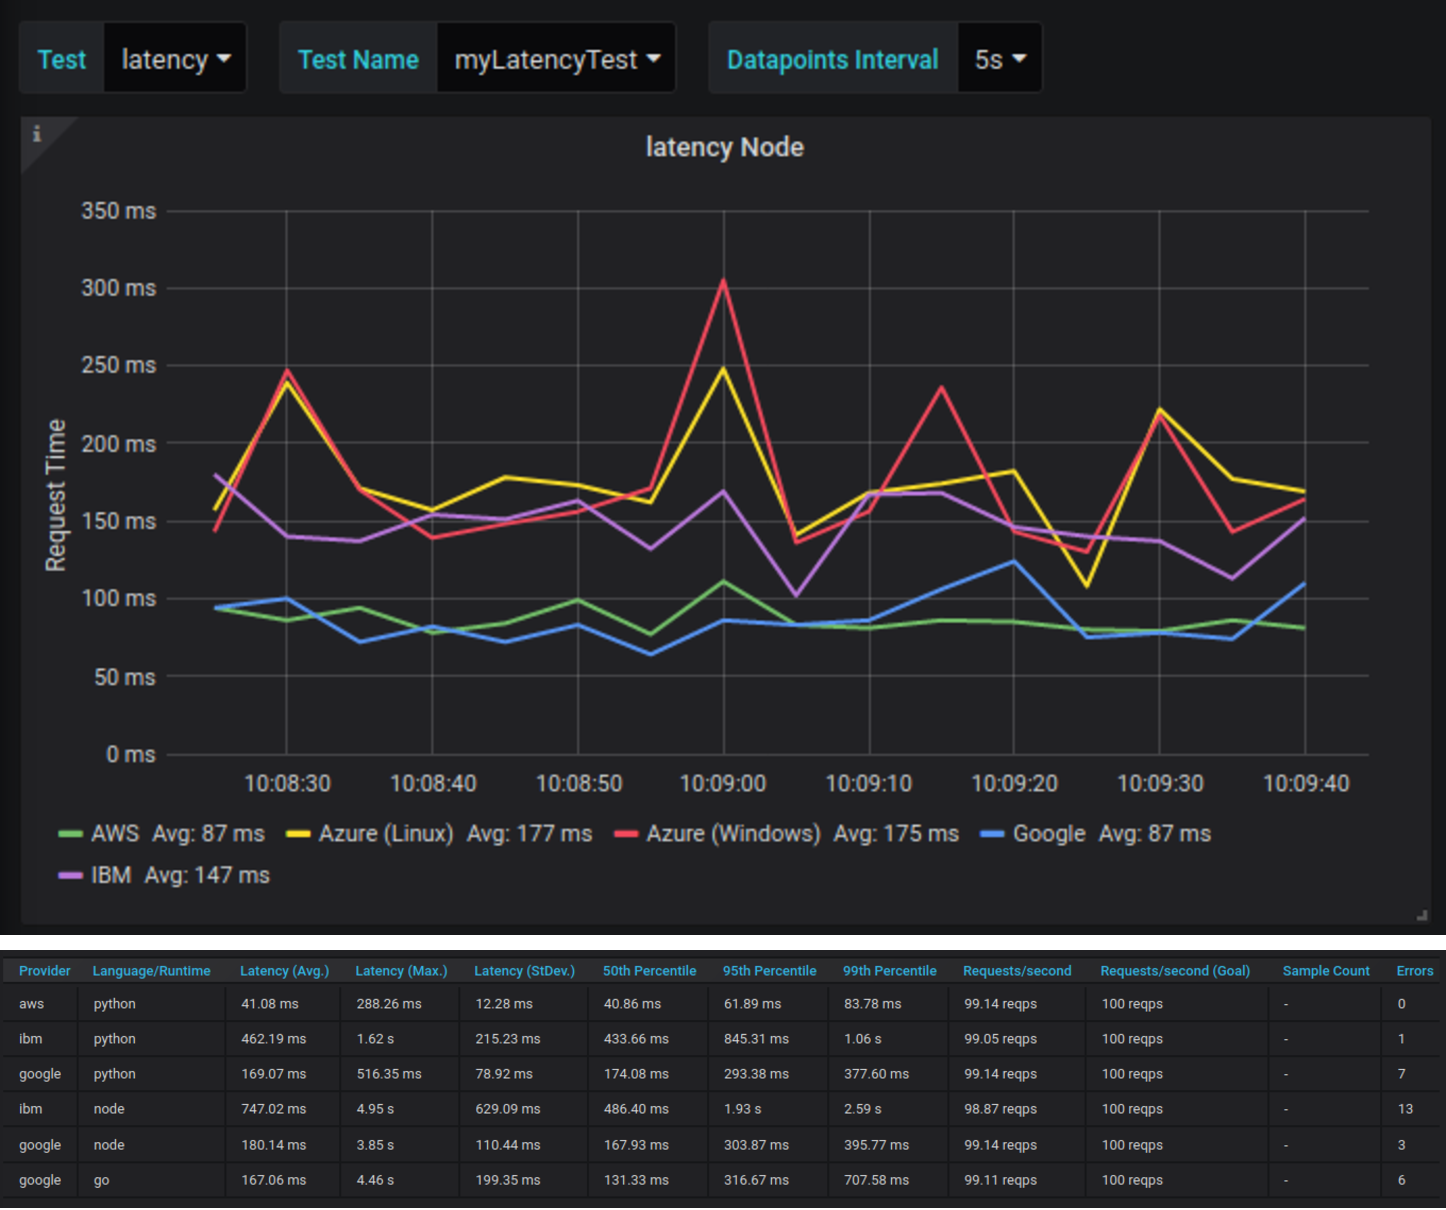
\includegraphics[width=0.48\textwidth]{bilder/grafana_combined}
\caption{Visualization of performance results in Grafana.}
\label{fig:grafana}
\end{center}
\end{figure}

%The plots can be grouped by cloud provider or by runtime. 
%There is a predefined Grafana dashboard for both options, the user can switch depending on his interests. 

%An example result of a general test can be seen in section \ref{sec:general_test}.

%\begin{figure*}[!t]
%\begin{center}
%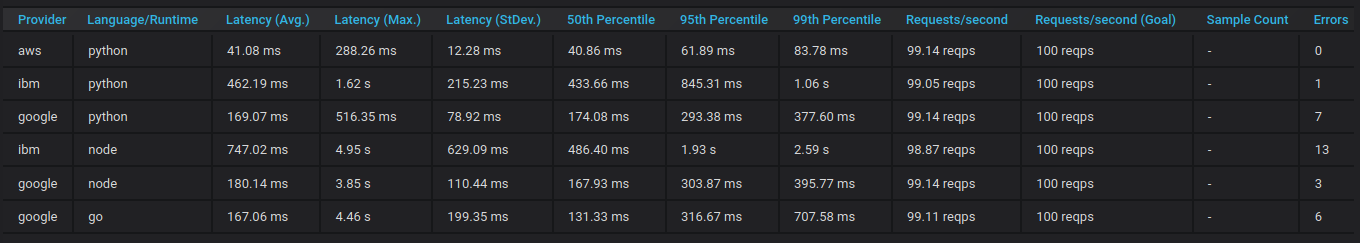
\includegraphics[width=1\textwidth]{bilder/benchmark_table.png}
%\caption[Benchmark results in Grafana]{Benchmark results in Grafana.}
%\label{fig:benchmark_table}
%\end{center}
%\end{figure*}

\subsection{Benchmarking}

For evaluating the performance of a deployed function, \sys's benchmarking component injects specific workloads toward the function exposed by a given serverless provider.
Our design is modular and currently supports \sloppy{\texttt{wrk2}~\cite{wrk2}}, a constant throughput, correct latency HTTP benchmarking tool. 
Additional tools are easy to integrate by providing a Docker container and a simple REST interface to exchange parameters and results. 
The \sys architecture allows users to directly visualize and analyze these results, using Grafana (\autoref{fig:grafana}) or other tools that can fetch the result data from the \gls{TSDB}.
%mainly relies on the wrk2 image. The parameters can be set in the web interface but they are basically just forwarded to wrk2. For the benchmark itself the user can choose the following parameters: requests per second, duration of the benchmark and the desired test to run e.g. the \gls{CPU} factors test. 
%Afterwards the load test will start and benchmark the chosen function on each cloud and runtime it was deployed to. 
%This process has to run sequentially otherwise the host of the benchmark suite could potentially not handle the load. 
%After the test has completed results will be parsed and inserted into the database and can be viewed as a table in Grafana. Figure \ref{fig:benchmark_table} shows an excerpt of a result.

% \subsection{Cleanup}

% Upon cleanup, all deployed functions are permanently deleted, as well as all the configurations and resource groups created at deployment time.
% and \gls{API} gateways on \gls{AWS} and IBM, all resource groups with a name containing latency, factors, matrix, filesystem and custom and on Google all functions in the configured project. 
%It should therefore be used very carefully and ideally with separate accounts only for this purpose.

%A more detailed test example with increasing load is discussed in section \ref{sec:loadtest}.

\subsection{Billing Costs Calculator}
\label{ssec:billingcalc}

\sys provides a pricing calculator component, which can be used to evaluate beforehand the cost of executing a certain workload on the supported cloud providers. 
%It does so either by setting the corresponding parameters manually or by exploiting results from previous executions.
%This component can be used to predict the cost of executing a given benchmark on a specific cloud provider.
Developers provide the planned workload (\eg number of function invocations, execution time per call, size of the returned data and allocated memory, \etc).
The \sys prototype produces an overview of the billing costs across the various serverless providers.
In future work, we envision this module to be able to forecast the billing costs even for full-fledged serverless applications, by applying machine-learning techniques to the system traces produced from sample executions serving real-world workloads.
%The prices for all clouds will be calculated and displayed in a table. 
%The functionality is basically the same as the pricing calculators provided by the cloud providers, except here all is in one place and directly comparable.
%Furthermore, the calculator takes the performed tests into account. 
%One can select a previously run test, select a runtime and then one only needs to provide the estimated number of invocations per month. 
%The calculation will happen by taking the execution time from the test results which of course can vary quite a lot between cloud providers and runtimes. 
%This method allows a much better approach of estimated cost. 
%In section \ref{sec:pricing} the same example will be explained and calculated for both hypothetical and with actual test results as input.

\subsection{Container Implementation}
\label{ssec:impl}

The implementation of \sys extensively relies on Docker containers.
Specifically, the main container invokes other containers using a technique called \emph{Docker-in-Docker}.\footnote{\url{https://www.docker.com/blog/docker-can-now-run-within-docker/}}
We do so by granting the main container access to \texttt{/var/run/docker.sock} and mounting it as a volume.
During our evaluation, we did not observe any particular performance degradations using this approach.

The implementation of \sys is freely available to the open-source community at \url{https://github.com/faas-benchmarking/faasdom}.
Its core components consist of about 2,000 lines of Node.js code.
%!TEX root = main.tex
\section{The \sys Benchmark Suite}\label{sec:tests}
The \sys benchmark suite currently consists of few tests which differ on the system aspect being stressed.
While some difference might be needed to comply with the different discrepancies across the cloud providers, the code executed is largely the same for all of them.
All functions are implemented using an \gls{HTTP} trigger, a common mean supported by all the supported serverless providers.
Currently, \sys includes:
\begin{itemize}
\item \texttt{faas-fact} and \texttt{faas-matrix-mult}: two CPU-bound benchmarks, respectively to factorize an integer and to multiply large integer matrices;
\item \texttt{faas-netlatency}: it immediately returns upon invocation, with a small \gls{JSON} \vs{MAISSEN: how small exactly? how many Bytes?}. This test is network-bound and useful to verify the roundtrip times for geographically distibuted deployments;
\item \texttt{faas-diskio}: an IO-bound benchmark to evalute the performance of a disk. Perhaps surprisingly, each serverless cloud provides a temporary file system that functions can use to read/write intermediate results. 
%The function can for example write a file with some intermediate results which it will later read again for further use. 
Other function calls which run in the same instance share this file system and can access the same file. %Given that serverless tends to be or should be stateless, the feature of a temporary storage is not of great importance. 
%Nevertheless, specific applications might benefit from such a feature and therefore it is included in this thesis. 
I/O operations are typically expensive \vs{MAISSEN: any link to online catalogue of prices to show this?} %and in a synchronous function that can lead to \gls{CPU} wait.
\item \texttt{faas-custom}: our design allows developers to easily implement custom functions. 
The suite provides templates for the currently supported cloud providers and the supported implementation languages. 
In the long term, we expect the number of custom functions to greatly outnumber the ones provided by the suite itself.
%Last but not least there is a customizable test. The objective of this test is that the user can easily implement his own function and then benchmark it. The skeleton is provided for each one of the four clouds in each of the four languages. A timer is included to measure the execution time which can later be further analysed.
\end{itemize}



%This section will briefly explain all the implemented test functions, what they test and how they are implemented. 
%All the functions are implemented with a \gls{HTTP} trigger, since it is one that all clouds support and is the easiest to test across all platforms. 
%For the same programming language and the same test, the implementation will vary from cloud to cloud a little bit. 
T%his is due to slightly different function calls and return statements each cloud defines on their own. However, these differences are not relevant regarding performance results.
%\subsection{Latency Test}
%\label{subsec:latency}
%The latency test  is fairly simple. 
%The function is called and then immediately returns a small \gls{JSON} body with \gls{HTTP} status code 200. The test function is intended to be as fast and simple as possible to measure latency for each cloud and runtime. 
%The following code listing \ref{code:latency} shows exemplary the implementation of the latency test on \gls{AWS} in Node.js.
%
%\begin{minipage}{\linewidth}
%\lstset{escapeinside={<@}{@>}}
%\begin{lstlisting}[frame=single,caption={Latency test implementation on AWS in Node.js},label=code:latency,linewidth=.82\textwidth,xleftmargin=.18\textwidth]
%  exports.handler <@\textcolor{javascriptbrown}{=}@> <@\textcolor{javascriptpurple}{function}@>(<@\textcolor{javascriptblue}{event}@>, <@\textcolor{javascriptblue}{context}@>, <@\textcolor{javascriptblue}{callback}@>) {
%      <@\textcolor{javascriptpurple}{const}@> <@\textcolor{javascriptblue}{res}@> <@\textcolor{javascriptbrown}{=}@> {
%          statusCode: <@\textcolor{javascriptroyalblue}{200}@>,
%          headers: {
%              <@\textcolor{javascriptred}{'Content-Type'}@>: <@\textcolor{javascriptred}{'application/json'}@>
%          },
%          body: JSON.stringify({
%              success: <@\textcolor{javascriptpurple}{true}@>,
%              payload: {
%                  <@\textcolor{javascriptred}{'test'}@>: <@\textcolor{javascriptred}{'latency test'}@>,
%              }
%          })
%      };
%    <@\textcolor{javascriptblue}{callback}@>(<@\textcolor{javascriptpurple}{null}@>, <@\textcolor{javascriptblue}{res}@>);
%  }
%\end{lstlisting}
%\end{minipage}
%
%\subsection{CPU Test (Factorization)}
%\label{sec:factors_test}
%This test describes the first of the two \gls{CPU} tests. 
%The \gls{CPU} is the component of a system which does effectively do the calculations of a program. 
%It is therefore the most important criterion of serverless computing and logically also the most expensive. This test is targeting mostly the \gls{CPU} by calculating all integer factors/divisors imperatively of an integer number. 
%Listing \ref{code:factors} shows pseudo code of such a number factorization.
%
%\begin{minipage}{\linewidth}
%\lstset{escapeinside={<@}{@>}}
%\begin{lstlisting}[frame=single,caption={Factorization test pseudo code},label=code:factors,linewidth=.75\textwidth,xleftmargin=.25\textwidth]
%  for(i = 1; i < SquareRoot(Number), i++) {
%      if(Number modulo i == 0) {
%          factors.add(i)
%          if(Number / i != i) {
%              factors.add(Number / i)
%          }
%      }
%  }
%\end{lstlisting}
%\end{minipage}
%
%The algorithm works as follows: one iterates from 1 to the square root of the number $N$ to be factorized. For each value $i$ it is tested if $N$ is dividable by $i$ without rest (modulo operator). If so, a factor of $N$ has been found and $i$ is added to the results. In addition, if $N$ divided by $i$ does not equal $i$ itself, the matching part $x$ of $i$ has also been found where $x \cdot i = N$. This is also the reason why only the numbers up to the square root of $N$ need to be considered. The algorithm has a complexity of $\mathcal{O}(n^{\frac{1}{2}})$.
%
%%\begin{remark}
%%The algorithm is not to be confused with prime factorization. In this case, all factors of a number are calculated but with prime factorization only prime numbers are calculated. 
%%The approach and results share some characteristics.
%%\end{remark}
%
%\subsection{CPU Test (Matrix Multiplication)}
%The matrix multiplication is the second \gls{CPU} test in this benchmark suite. 
%The user can input a number $n$ which defines the width and height of two matrices. The two matrices are both filled with random integer numbers between 0 and 100. 
%The product of those two matrices is calculated by multiplication. The algorithm is defined in listing \ref{code:matrix} in pseudo code.
%
%\begin{minipage}{\linewidth}
%\lstset{escapeinside={<@}{@>}}
%\begin{lstlisting}[frame=single,caption={Matrix multiplication test pseudo code},label=code:matrix,linewidth=0.8\textwidth,xleftmargin=.2\textwidth]
%  matrixA = randomMatrix[n][n]
%  matrixB = randomMatrix[n][n]
%  matrixMult = [n][n];
%  
%  for(i = 0; i < matrixA.height; i++) {
%      for(j = 0; j < matrixB.width; j++) {
%          sum = 0;
%          for(k = 0; k < matrixA.width; k++) {
%              sum += matrixA[i][k] * matrixB[k][j];
%          }
%          matrixMult[i][j] = sum;
%      }
%  }
%\end{lstlisting}
%\end{minipage}
%\newline
%
%First, two matrices of height and width $n$ are defined and filled with random integer numbers from 0 to 100. Also an empty matrix for the result is initialized. For each field of the resulting matrix one needs to calculate the dot product of row $i$ from matrix $A$ and column $j$ of matrix $B$. This is achieved by multiplying each field of row $i$ from matrix $A$ with each field of column $j$ from matrix $B$ and accumulating the sum over $k$. The sum is then stored as field $i,j$ in the resulting matrix. The algorithm has a complexity of $\mathcal{O}(n^{3})$.
%\subsection{I/O Test}
%The fourth test in this benchmark suite is a disk test. 
%Each serverless cloud provides a temporary file system which the functions can use. 
%The function can for example write a file with some intermediate results which it will later read again for further use. 
%Other function calls which run in the same instance share this file system and can also access the file. Given that serverless tends to be or should be stateless, the feature of a temporary storage is not of great importance. 
%Nevertheless, specific applications might benefit from such a feature and therefore it is included in this thesis. 
%I/O operations are often expensive and in a synchronous function that can lead to \gls{CPU} wait.
%%The implementation of the test is fairly simple. Listing \ref{code:filesystem} shows the pseudo code of the test.
%
%
%\begin{minipage}{\linewidth}
%\lstset{escapeinside={<@}{@>}}
%\begin{lstlisting}[frame=single,caption={I/O test pseudo code},label=code:filesystem,linewidth=0.75\textwidth,xleftmargin=.25\textwidth]
%  text = ""
%    
%  for(i = 0; i < s; i++) {
%      text += "A";
%  }
%  
%  startWrite = Time.Now()
%  for(i = 0; i < n; i++) {
%      writeFile(i+'.txt', text, 'utf-8');
%  }
%  endWrite = Time.Now()
%  
%  startRead = Time.Now()
%  for(i = 0; i < n; i++) {
%      file = readFile(i+'.txt', 'utf-8');
%  }
%  endRead = Time.Now()
%  
%  writeTime = endWrite - startWrite
%  readTime = endRead - startRead
%\end{lstlisting}
%\end{minipage}
%\newline

%The algorithm writes files and then reads them. 
%It takes two input parameters $n$ defining the number of files and $s$ the size of each file in bytes. 
%A string \texttt{text} is generated with length equal to $s$. 
%Since the encoding used is \texttt{utf-8} each normal character takes 8 bits or 1 byte of storage. 
%Then $n$ many files are written to the file system. 
%After that all the written files are read. 
%Both these operations are timed and the result will be the time it took to write respectively read the files.
%The complexity of the algorithm is $\mathcal{O}(n)$.

%\subsection{Custom Test}
%Last but not least there is a customizable test. The objective of this test is that the user can easily implement his own function and then benchmark it. The skeleton is provided for each one of the four clouds in each of the four languages. A timer is included to measure the execution time which can later be further analysed.
%!TEX root = main.tex
\section{Evaluation}
\label{sec:evaluation}
Rather than presenting an evaluation of the \sys internal components, this section presents the typical evaluation results users can achieve by using \sys.
We carried out these tests between \vs{MAISSEN: insert start date} and \vs{MAISSEN: insert end date}.
We designed these experiments to answer the following questions: 
\emph{(1)} what is the most effective programming language to use for serverless applications;
\emph{(2)} what is the most convenient provider; 
and \emph{(3)} which provider provides the most predictable results.

%chapter results of performed tests will be presented and explained, an example for a pricing calculation will be given, the services among the cloud providers will be compared and some general advantages and disadvantages about serverless computing will be specified derived from these results.
%
%In this thesis, four different tests have been performed. Each one will be discussed in detail and results will be presented in the following subsections.

\begin{figure*}[!t]
\centering
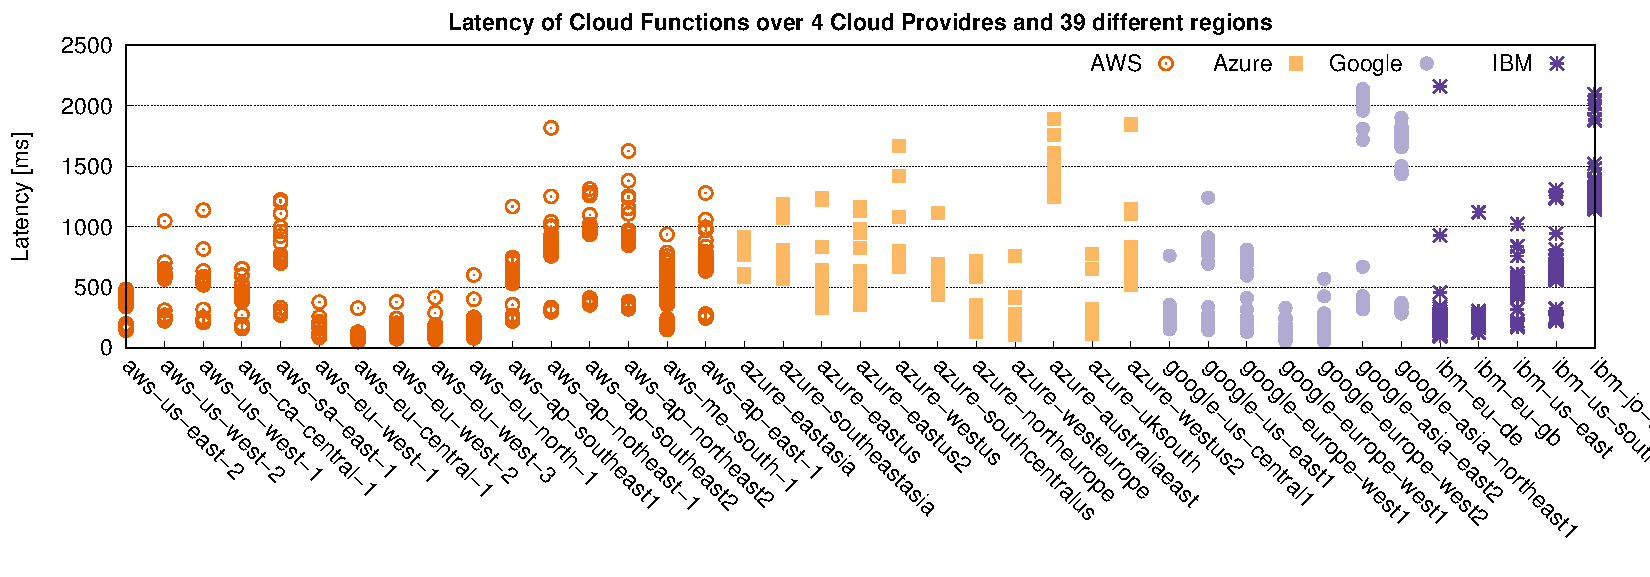
\includegraphics[width=1.0\textwidth]{bilder/latency/latency.pdf}
\caption{Latency test scatter plot. At the time of our experiment, \texttt{azure-west-us}  had issues deploying Node.js, hence we resort to \texttt{.NET}.}
\label{fig:latency_plot}
\end{figure*}

\subsection{Benchmark: Latency}
In this test, we measure the latency (round-trip) for all cloud providers and corresponding regions, using the \texttt{faas-netlatency} benchmark.
%This test differs from a normal ping, that effectively a cloud function is executed instead of just returning a message on a more abstract level. 
Unless specified otherwise, we deploy the Node.js version of the test using 128\gls{MB}.
With the exception of \textit{aws-australia-east}, we deploy Linux \vs{MAISSEN: version/distribution}.   
%The test was performed in Node.js with 128\gls{MB} of memory (Azure 1.5\gls{GB}) with the latency test described in section \ref{subsec:latency}. 
Every 5 seconds, a requests was sent to each cloud and region until a sample size of 100 was obtained. 
Figure~\ref{fig:latency_plot} reports our results. 
%This test was carried out from Bern, Switzerland.
%\begin{remarks}
%\text{ }
%\begin{itemize}
%    \item For Azure, this test was only done with Linux as underlying OS. The OS should not matter in regards to latency.
%    \item The \textit{westus} region of Azure had problems deploying it in Node.js and therefore .NET was used. Following error was produced: \texttt{The scale operation is not allowed for this subscription in this region. Try selecting different region or scale option.}\\
%    Also trying to create the function in the Azure portal failed and an error was indicated but the error message could not be viewed.
%    \item On Azure region \textit{australiaeast} the function could not be deployed, although no error was risen. Therefore it was deployed on Windows instead of Linux.
%\end{itemize}
%\end{remarks}
%The graphic \ref{fig:latency_plot} shows a scatter plot with the results of the test.
\vs{MAISSEN: here we need a short discussion on the results. Something like the following, can you complete ? I'll check afterwards}.
We observe the following.
We achieve the lowest latency on \vs{MAISSEN: FIX}, about \vs{MAISSEN: FIX}, and the highest of \vs{FIX}. 
The average latency is \vs{MAISSEN: FIX}.
Finally, the best performing cloud provider is \vs{MAISSEN: FIX, explain}.

%For more detailed results see table \ref{tab:latency}. 
%The raw result file, R script and plot image are also on \href{https://github.com/Bschitter/benchmark-suite-serverless-computing/tree/master/results/1-latency}{GitHub}.

\subsection{Benchmark: Cold/Start}
\vs{STOPPED HERE}
\label{sec:coldstart}
%This test measured the cold start latency. 
A cold start happens when a function takes longer than usual to start up and execute. 
This occurs mostly after the deployment, when the function has not been used in a while\vs{MAISSEN: is it know how long is this period?} or when a new instance needs to be provisioned for scaling purposes. 
\vs{MAISSEN: can't understand this sentence, can you rephrase? In order for the cloud provider to get up the instance and deploy the specific code on it, some time can pass.} 
Figure~\ref{fig:azure_coldstart} shows the execution workflow for a cold start on Azure, as ooposed to the \emph{warm} case, but a similar workflow is valid on the other cloud providers.
\vs{MAISSEN: do you have the same results for the other providers? eg, why only Azure?}

\begin{figure}[htp]
\centering
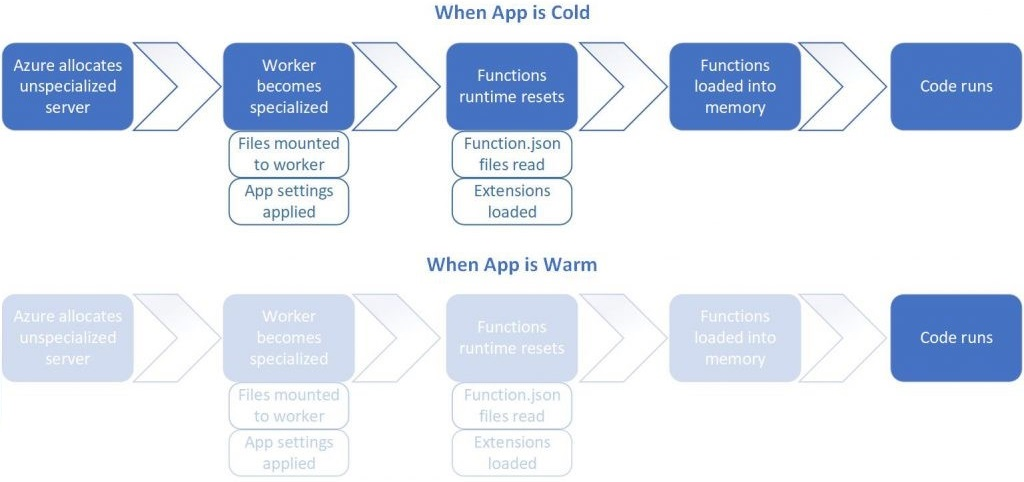
\includegraphics[width=0.4\textwidth]{bilder/azure-coldstart.jpeg}
\caption{Workflow for cold and warm start on Azure~\cite{AzureColdStart}\vs{Fig to be re-done}}
\label{fig:azure_coldstart}
\end{figure}

There are several steps to perform before a function can execute: allocate a server, setup a workier with the associated code, packages and extensions, load the function in memory, and finally run it.
When the function is warm, the function is ready and can just be invoked immediately. 

We execute each test ten times for each runtime and each cloud. 
Functions are executed using 512 \gls{MB} and without external packages, to reduce the baseline memory footprint (and the corresponding loading time) to the bare minimum.
%The cold start latency has been tested ten times for each runtime on each cloud.
%Memory size was defined with 512 \gls{MB} and no packages were loaded into the function. 
We executed these tests on the following regions: \texttt{eu-central-1} for AWS,  \texttt{west-europe} for Azure,  \texttt{europe-west1} for Google and \texttt{eu-de} for IBM. 
Note however that chosen region has no impact the cold start latency. 
We compute the cold start latency as:
\begin{equation*}
(cold\ start\ latency) = (tot.\ req.\ time) - (normal\ avg.\ latency)
\end{equation*}

Figure~\ref{fig:coldstart_plot} reports our results using a box plot.
 \gls{AWS} is overall the fastest, with an average cold start latency of only 335 ms for Node.js, Python and Go. 
Using .NET achieves worse results, up to 1739 ms, possibly due to the nature and compilation of .NET respectively C\#. 
On Azure, cold start latency is strictly more than 2 seconds and up to 5 seconds, with the exception of the combination .NET on Windows, which averages at 1917 ms. 
Google compares similarly to \gls{AWS}.
Finally, \gls{IBM} consistenly produces  higher cold start latency, in the 2-3 seconds range. 
\gls{IBM} shows a similar pattern \vs{MAISSEN: can you clarify? you mean that the ranking of the results wrt to the languages is the same?} as \gls{AWS} although the cold start latency is around 600 ms higher for Node.js, Python and Go but similar for .NET.

\vs{MAISSEN: what is this 'reclying' you refer to ? can you clarify?}
On \gls{AWS} and \gls{IBM} it took usually around 10 minutes of no activity for the instance to be recycled by the provider; the same took up to 20 minutes on Azure. 
On Google, this time varied varied from 10 minutes up to 10 hours.

\begin{figure}[!t]
\centering
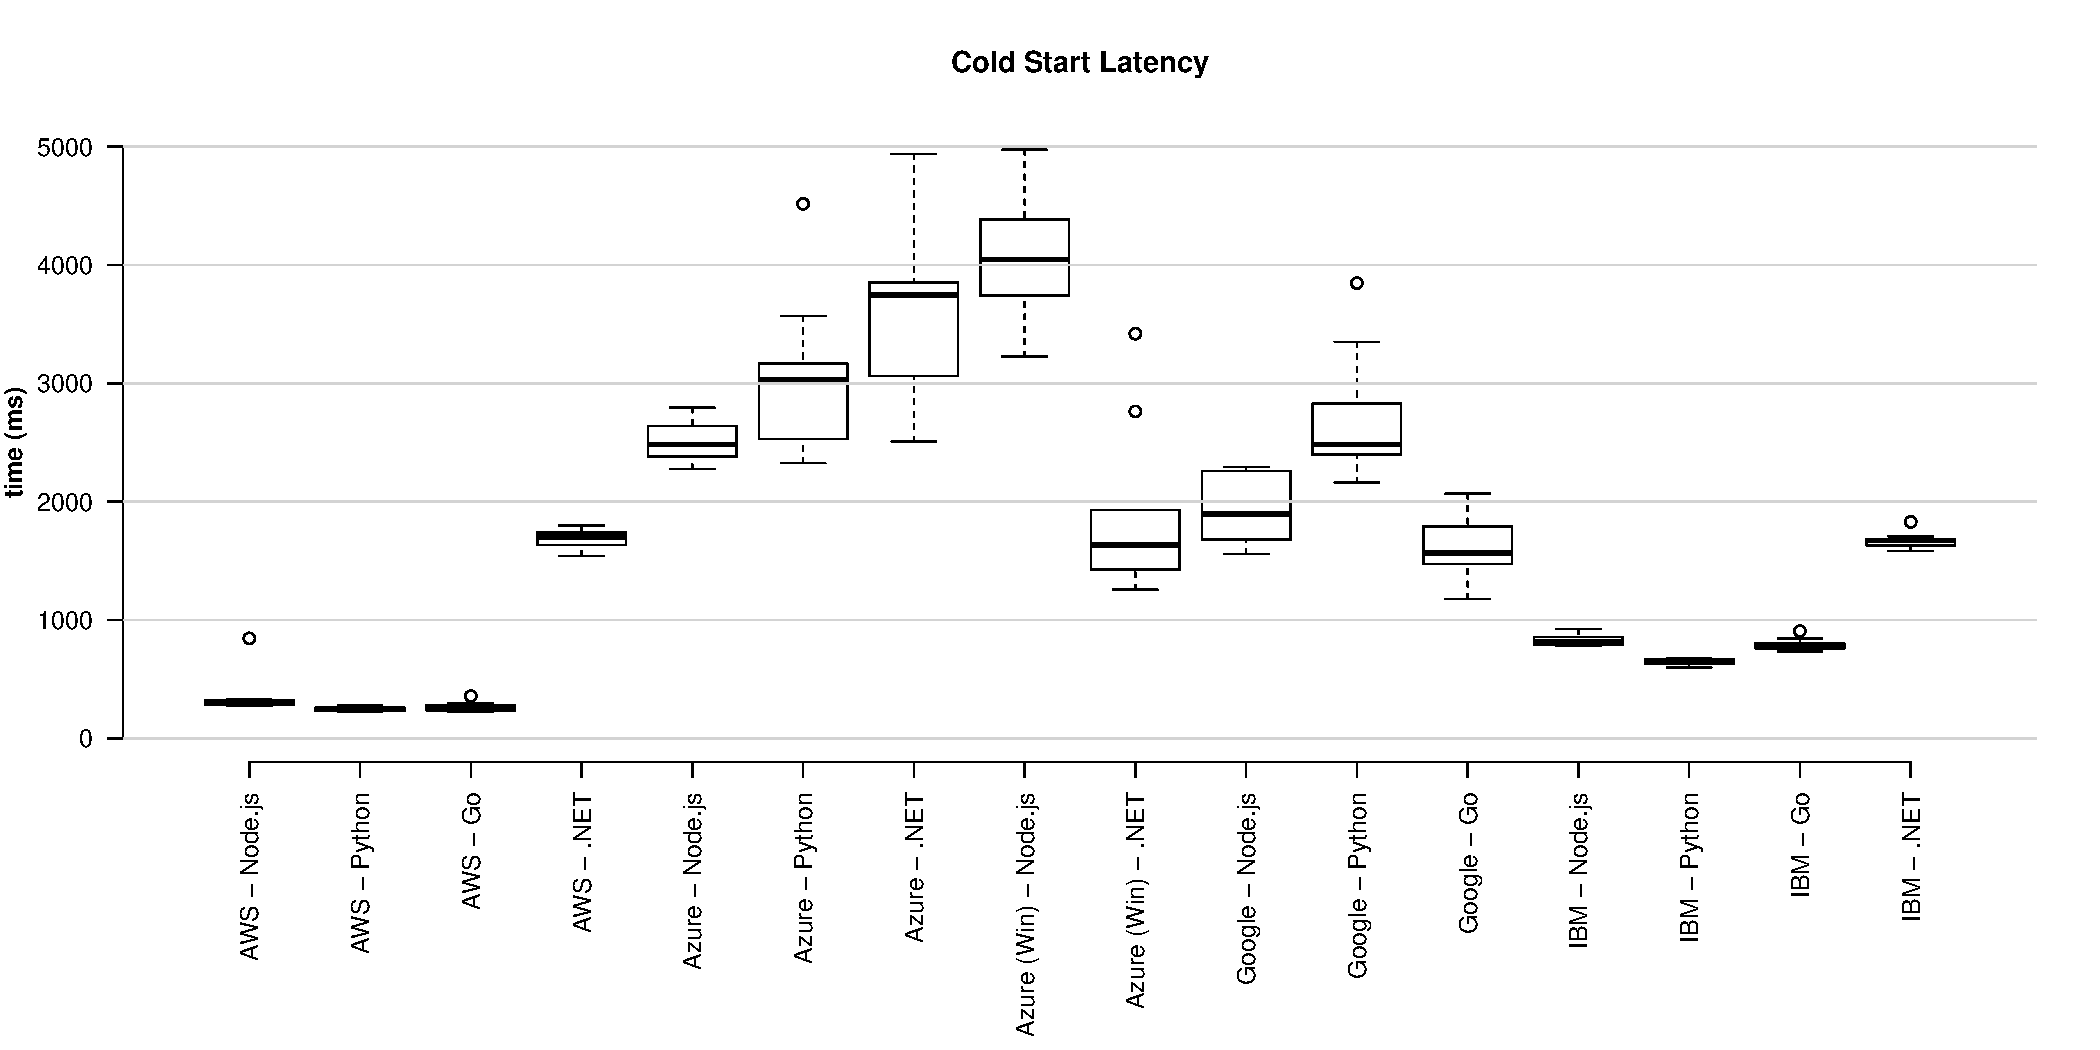
\includegraphics[width=0.5\textwidth]{bilder/cold_start/boxplot_coldstart_all.pdf}
\caption{Cold start latency.}
\label{fig:coldstart_plot}
\end{figure}



\subsection{Benchmark: CPU-bound functions}
\vs{find better section name}
\label{sec:general_test}
%This test was performed to analyze the functions under normal circumstances, meaning that there is not much load respectively that the load can be handled well by the cloud provider. The objective is to compare the achieved performance of the clouds regarding execution speed and the thereby implicated costs. 
This benchmark evaluates how CPU-bound workload behave across the different cloud providers.
% evaluation the \gls{CPU} factors test (see section \ref{sec:factors_test}) was executed. 
A function (\texttt{faas-fact}) is invoked every five seconds, using a large-enough integer as parameter. 
We collect 100 results for every configuration (runtime, memory, cloud provider).
%The function was invoked every five seconds until a sample size of $n=100$ was reached. 
%This for each \gls{MB} configuration, each runtime and each cloud. 
A%s input parameter $26'888'346'474'443$ was selected since with this number the function finished ahead of the timeout for low configurations and simultaneously was not too quickly finished for high configurations. 
Figure~\ref{fig:general_python_plot} depicts our result for Python.

\begin{figure}[!t]
\centering
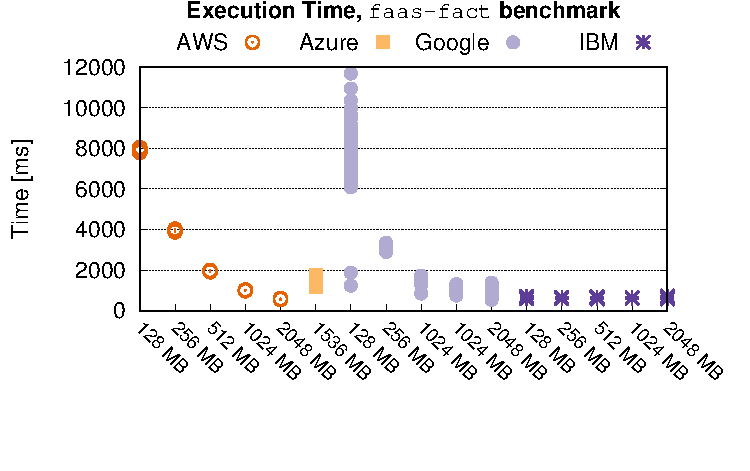
\includegraphics[width=0.5\textwidth]{bilder/general_python/cpufact.pdf}
\caption{Execution times of the \texttt{faas-fact} benchmark in Python. Azure allows only one single memory configuration (1536 MB)}
\label{fig:general_python_plot}

\end{figure}

We note few interesting facts.
On \gls{AWS} Lambda, the standard deviation is very low (\vs{MAISSEN: how much is the lowest?}), with very consistent execution times. 
As expected, every doubling of the allocated memory achieves halving of the execution time, performance scales linearly to allocated memory~\cite{AWSLambdaConfig}. 

Azure's memory configuration of 1536 \gls{MB} suggests its performance to be in the 1024-2048 \gls{MB} range.
Surprisingly, it is slower than 1024 \gls{MB} instances of the other clouds.  
Google Cloud Platform performs similarly to \gls{AWS}, although more scattered for 128 \gls{MB} of memory. 
Google achieves bette results for several memory configurations than \gls{AWS} (128, 256, 512 and 1024 \gls{MB}). % but not for 2048 \gls{MB}. For the first three times doubling the memory leads to halved execution time. 
Note however that the performance scaling behaves differently on the Google platform~\cite{GoogleFunctionsPricing}.
%But not entirely for the next two steps since Google does not scale \gls{CPU} completely linear to allocated memory \cite{GoogleFunctionsPricing}. 
The resuls we gathered on the \gls{IBM} platform suggests that memory allocation does not correlate with \gls{CPU} allocation in any way, with five different configurations perform very closely. 
This is remarkable since the pricing model of \gls{IBM} only accounts for GB-Seconds used. 
\vs{MAISSEN: Is this true for all the languages? These resuls are only for Phython. Do you have the same tests for all the other languges? This means that a user could deploy his application always with the smallest memory option possible and would thereby get the same performance for the smaller price.}
%The results and plots for this and the three other runtimes can be found on \href{https://github.com/Bschitter/benchmark-suite-serverless-computing/tree/master/results/3-general}{GitHub}.

\subsection{Benchmark: Throughput/Latency}
\label{sec:loadtest}
To understand the saturation point of the deployed services, we rely on \texttt{wrk2}~\cite{wrk2}, a constant throughput/exact latency HTTP-based benchmarking tool.
We design this benchmark to issue function call invocations at increasingly high request rates, from 10 up to 1000 req/sec.
For each of the configurations, \texttt{wrk2} reports the average latency to handle the requests (\emph{i.e.}, the functions).
Between each configuration, the benchmark waits for sufficient time to process potential pending requests in the queue.
Figure~\ref{fig:load_test_latency_all} shows our results for the \texttt{faas-matrix-mult} test function.
%The load test is designed to benchmark the serverless functions up to 1000 requests per second. 
%This is carried out with the \gls{HTTP} benchmark tool \textit{wrk2} (see \cite{wrk2}). A function is first called with 10 requests per second for the duration of 1 minute. 
%Subsequently with 25, 50, 100, 200, 400, 800 and finally 1000 requests per second each time for one minute. 
%In between is a short break of 10 seconds to allow the function to process requests that are still queued. As test, the matrix function with a parameter of 100 is used. With this setup the matrix function should have an average execution time of about 100ms for Node.js, Go and .NET and around 250ms for Python. The graphic \ref{fig:load_test_latency_all} displays the average latency results grouped by runtime.

\begin{figure*}[!t]
\centering
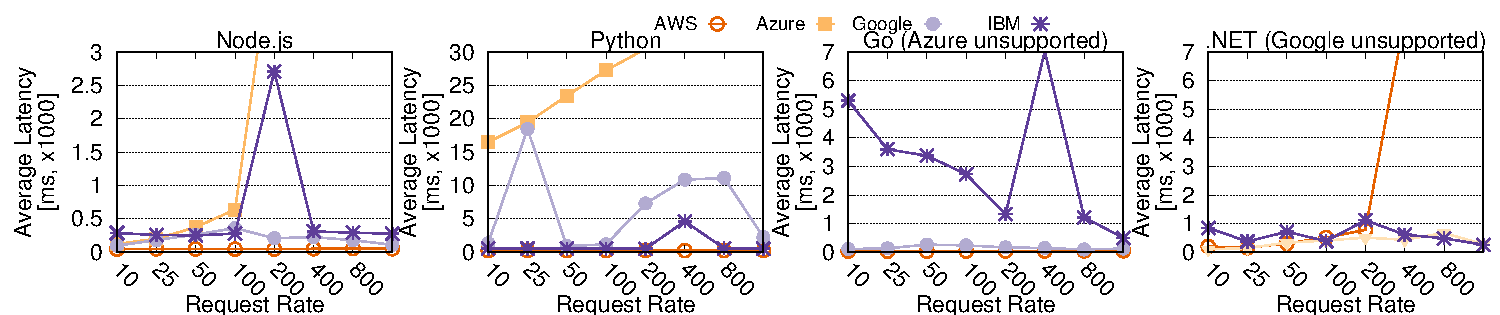
\includegraphics[scale=0.7]{bilder/loadtest_average_latency/tputlat_combined.pdf}
\caption{Load test average latency.}
\label{fig:load_test_latency_all}

\end{figure*}
\vs{STOPPED HERE}
The results are now discussed step by step. \gls{AWS} has for all four runtimes an extremely steady response latency throughout the increasing load. This is very remarkable and a very good result and can be probably traced back to the low cold start latency and the good and consistent performance presented in section \ref{sec:general_test}.\\
On Azure it looks quite different. Azure can handle the load on Windows as operating system. But in the first increasing steps from 10 to 100 or 200 RPS latency rises although it flattens out afterwards. On Linux, Azure performs very bad and can not scale out quickly enough to serve the requests in an acceptable time frame. The response time climbs more or less linearly to the amount of request per second sent. That is a strong indication that none or too few new instances are allocated to handle the load. At the time of 1000 requests per second one could see in the Azure portal Live Metrics Stream that e.g. for .NET only 12 instances have been deployed (see figure \ref{fig:live_metrics_stream}). Additionally the screenshot shows that only 500 requests per second get handled by the function, the rest is probably waiting in a queue.
\begin{remark}
In the screenshot the request duration differs from the wrk2 results since that is most likely only considering execution time without queuing time.
\end{remark}

\begin{figure}[htp]
\centering
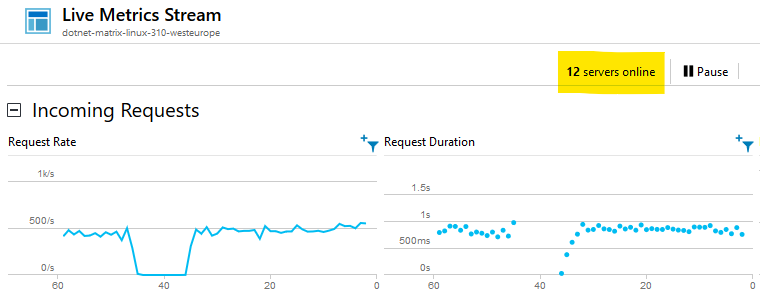
\includegraphics[scale=1.0]{bilder/Azure_Dotnet_1000.png}
\caption[Azure Linux .NET Live Metrics Stream during 1000 RPS]{Azure Linux .NET Live Metrics Stream during 1000 RPS\\Source: screenshot Azure portal}
\label{fig:live_metrics_stream}
\end{figure}

For Node.js and .NET the latencies went up to 24s respectively 18s and are not plotted in the graph for illustration purposes. On Python, Azure returned from 200 \gls{RPS} and above almost only \gls{HTTP} errors and the result of wrk2 is not representative and hence not plotted.\\
Google can manage the load generally well, although latency increases a little bit for Node.js and Go. With Python, Google has the biggest problems and seems overwhelmed when requests increase. It can not scale quickly enough and the average request duration increased from 1356ms to 18448ms with 10 \gls{RPS} respectively 25 \gls{RPS}. After that, this phenomena happens again but less drastically. This can possibly be explained by the fact that the function has a longer execution time in Python and Google can scale longer running functions less good. Overall the performance is good. Figure \ref{fig:google_graph_go} shows the number of instances allocated during the Go load test on Google.

\begin{figure}[htp]
\begin{center}
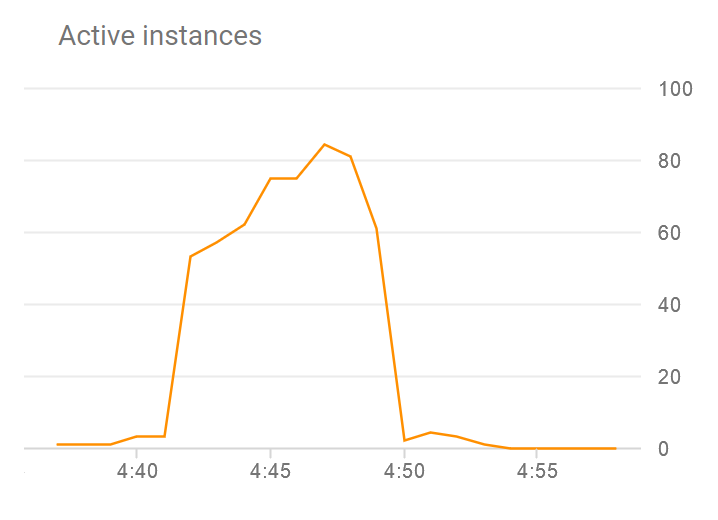
\includegraphics[width=0.5\textwidth]{bilder/Google_Go_Instances.png}
\captionsetup{justification=centering, labelfont=bf}
\caption[Google Go active instances during load test]{Google Go active instances during load test\\Source: screenshot Google cloud portal}
\label{fig:google_graph_go}
\end{center}
\end{figure}

Lastly, the result of \gls{IBM} will be discussed. Those outcomes differ from the others relatively much. On Node.js and .NET it can roughly keep up to the competition but operates a little slower and on Node.js it has a striking outlier. The Python function on IBM nearly performs as well as on \gls{AWS}, but the same cannot be said about Go. The Go runtime performed much slower in the load test as with the competitors, although as seen in the cold start test in section \ref{sec:coldstart} it has a similar cold start latency as Node.js and Python and as shown in the appendix table \ref{tab:general} it performs generally well on Go. Thus this bad performance cannot be derived from this or other tests and it is possible that IBMs auto scaling mechanism does not work well for Go. Of the amount of instances deployed, IBM delivers no statistics.\\
So far, the latency has been examined and now the actual throughput will be explained. Most of the cloud providers and runtimes could handle the load and only had an irrelevant smaller throughput than tested against. Therefore only significant impacts in throughput will be presented, meaning that the throughput was less than 90\% of the tested one. The subsequent table \ref{table:rps} shows where throughput was below 90\%.
In addition, there are detailed result plots (figure \ref{fig:loadtest_percentile_node} - \ref{fig:loadtest_percentile_dotnet}) and tables (table \ref{table:aws_load_test} - \ref{table:ibm_load_test}) in the appendix.
\begin{table}[htp]
\centering
\captionsetup[table]{justification=centering, labelfont=bf}
\scalebox{0.93}{\begin{tabular}{l|l|r|r|r} 
\textbf{Cloud} & \textbf{Runtime} & \textbf{RPS (goal)} & \textbf{RPS (actual)} & \textbf{RPS in \%} \\ \hline
Azure & Node.js & 200 & 179 & 89.50\% \\ \hline
Azure & Node.js & 400 & 227 & 56.75\% \\ \hline
Azure & Node.js & 800 & 278 & 34.75\% \\ \hline
Azure & Node.js & 1000 & 327 & 32.70\% \\ \hline
Azure & Python & 10 & 6 & 60.00\% \\ \hline
Azure & Python & 25 & 12 & 48.00\% \\ \hline
Azure & Python & 50 & 18 & 36.00\% \\ \hline
Azure & Python & 100 & 25 & 25.00\% \\ \hline
Azure & Python & 200 & 30 & 15.00\% \\ \hline
Azure & Python & 400 & 15 & 3.75\% \\ \hline
Azure & Python & 800 & 14 & 1.75\% \\ \hline
Azure & Python & 1000 & 15 & 1.50\% \\ \hline
Azure & .NET & 400 & 324  & 81.00\% \\ \hline
Azure & .NET & 800 & 407 & 50.88\% \\ \hline
Azure & .NET & 1000 & 512 & 51.20\% \\ \hline
Google & Python & 25 & 12 & 48.00\% \\ \hline
Google & Python & 200 & 168 & 84.00\% \\ \hline
Google & Python & 400 & 297 & 74.25\% \\ \hline
Google & Python & 800 & 575 & 71.88\% \\ \hline
IBM & Go & 25 &  21 & 84.00\% \\ \hline
\end{tabular}}
\caption[Load tests that achieved less than 90\% of RPS]{Load tests that achieved less than 90\% of RPS}
\label{table:rps}
\end{table}

\subsection{Pricing}
\label{sec:pricing}
In this section two pricing examples will be calculated and explained. The first one will be theoretical and the second one will be based on the general test in section \ref{sec:general_test}. Table \ref{table:pricing} shows the prices per unit for each cloud. Prices on \gls{AWS} and Azure can vary depending on the location. The table and the examples use the prices of the region \texttt{eu-central1} for \gls{AWS} and \texttt{westeurope} for Azure. All clouds round up GB-Seconds and GHz-Seconds up to the next 100ms per invocation, except for Azure which rounds it up to the next 1ms.

\begin{table}[htp]
\centering
\captionsetup[table]{justification=centering, labelfont=bf}
\begin{tabular}{l|l|l|l|l} 
         & \textbf{per invocation} & \textbf{per GB-Second} & \textbf{per GHz-Second} & \textbf{per GB network egress} \\ \hline
\textbf{AWS}      &  0.0000002  &  0.000016667 &  -       & 0.09 \\ \hline
\textbf{Azure}    &  0.0000002  &  0.000016    &  -       & 0.087 \\ \hline
\textbf{Google}   &  0.0000004  &  0.0000025   &  0.00001 & 0.12 \\ \hline
\textbf{IBM}      &  -          &  0.000017    &  -       & - \\
\end{tabular}
\caption[Serverless functions pricing]{Serverless functions pricing, all prices in USD as of 22.01.2020\\ Data source: \cite{AWSPricing, AzurePricing, GoogleFunctionsPricing,IBMPricing}}
\label{table:pricing}
\end{table}

As one can see Google seems to be to have the most sophisticated pricing model of all. Charging exactly for not only the GB-Seconds used but also the GHz-Seconds. The pricing model of \gls{AWS} and Azure are very similar and the one of \gls{IBM} only takes into account GB-Seconds and they are not significantly more expensive.\\
All of the cloud have a certain free tier quantity which is included per month. Table \ref{table:free_tier} lists the free quantities. Network egress free tier is shared with all network egress of the cloud. Free tier is not considered in the following two examples.

\begin{table}[htp]
\centering
\captionsetup[table]{justification=centering, labelfont=bf}
\begin{tabular}{l|l|l|l|l} 
         & \textbf{Invocations} & \textbf{GB-Seconds} & \textbf{GHz-Seconds} & \textbf{GB network egress} \\ \hline
\textbf{AWS}      &  1'000'000  &  400'000     &  -       & 1 \\ \hline
\textbf{Azure}    &  1'000'000  &  400'000     &  -       & 5 \\ \hline
\textbf{Google}   &  2'000'000  &  400'000     &  200'000 & 5 \\ \hline
\textbf{IBM}      &  -          &  400'000     &  -       & - \\
\end{tabular}
\caption[Serverless functions free tier]{Serverless functions free tier as of 22.01.2020\\Data source: \cite{AWSPricing, AzurePricing, GoogleFunctionsPricing,IBMPricing}}
\label{table:free_tier}
\end{table}

\subsection*{Example 1}
Let's assume a company has a custom application for image processing written in Python. It does some modifications to the image and then saves the result in a storage solution of the correspondent cloud. Each month around 10 million images are processed. This task is not time critical but should be cost efficient. On a developers desktop computer the task takes around 5 seconds to complete and uses up to 450 \gls{MB} of memory. On a cloud platform a similar result is expected. In this example there is no network egress.
\subsubsection*{Calculation}
\begin{align*}
\text{\textbf{Cloud}}&: \text{\textbf{Invocations}} &+\quad& \text{\textbf{GB-Seconds}} &+\quad& \text{\textbf{GHz-Seconds}} &=\quad& \text{\textbf{Cost}} \\
\text{AWS}&: 10\text{M} \cdot 0.0000002 \$ &+\quad& 10\text{M} \cdot 0.5 \cdot 5 \cdot 0.000016667 \$ & & &=\quad& 418.675 \$ \\ 
\text{Azure}&: 10\text{M} \cdot 0.0000002 \$ &+\quad& 10\text{M} \cdot 0.5 \cdot 5 \cdot 0.000016 \$ & & &=\quad& 402.000 \$ \\
\text{Google}&: 10\text{M} \cdot 0.0000004 \$ &+\quad& 10\text{M} \cdot 0.5 \cdot 5 \cdot 0.0000025 \$ &+\quad&  10\text{M} \cdot 0.8 \cdot 5 \cdot 0.00001 \$ &=\quad& 466.500 \$ \\
\text{IBM}&:  &+\quad& 10\text{M} \cdot 0.5 \cdot 5 \cdot 0.000017 \$ & & &=\quad& 425.000 \$ \\ 
\end{align*}

As one can see the cheapest in this case would be Azure, followed by \gls{AWS}, \gls{IBM} and finally Google as the most expensive. With that amount of invocations and execution time all clouds are comparable.\\
Now the problem with this calculation is that it only assumes the execution times on the clouds which is the most essential part of the pricing calculation. Some clouds may perform much better than others. Example 2 will take actual execution time into consideration.
\subsection*{Example 2}
This example takes the result of the \gls{CPU} factors test of section \ref{sec:general_test} as a basis. This test is also in the runtime Python. Let's also assume 10 million function calls are invoked per month. With the fixed parameter of $26'888'346'474'443$ the function should not consume more than 100 \gls{MB} of memory. Its return size is around 4 KB per call. As execution times we take the average (rounded up to 100ms if applicable) of the result.
\begin{remark}
Azure claims that it only charges the GB-Seconds the function actually used, rounded up to the next 128 \gls{MB} step \cite{AzurePricing}. It seems therefore that the pricing model of Azure is similar to the one of \gls{IBM}, delivering the same performance independent of memory size.
\end{remark}
Doing the equivalent calculations as in example 1, the following results are obtained as shown in table \ref{table:example2}.

\begin{table}[htp]
\centering
\captionsetup[table]{justification=centering, labelfont=bf}
\begin{tabular}{|l|r|r|r|r|r|r|} \hline
     &   \textbf{Rounded time}  & \textbf{Invocation} & \textbf{GB-Seconds} & \textbf{GHz-Seconds} & \textbf{Network} & \textbf{Total} \\ \hline
AWS  128MB      & 8000ms&  2.00\$  &  166.67\$     &  -        & 3.43\$ & 172.10\$ \\ \hline
AWS  256MB      & 4000ms&  2.00\$  &  166.67\$     &  -        & 3.43\$ & 172.10\$ \\ \hline
AWS  512MB      & 2000ms&  2.00\$  &  166.67\$     &  -        & 3.43\$ & 172.10\$ \\ \hline
AWS 1024MB      & 1000ms&  2.00\$  &  166.67\$     &  -        & 3.43\$ & 172.10\$ \\ \hline
AWS 2048MB      &  600ms&  2.00\$  &  200.00\$     &  -        & 3.43\$ & 205.43\$ \\ \hline
Azure 128MB     & 1267ms&  2.00\$  &   25.34\$     &  -        & 3.32\$ &  30.66\$ \\ \hline
Google  128MB   & 7700ms&  4.00\$  &   24.06\$     &  154.00\$ & 4.58\$ & 186.64\$ \\ \hline
Google  256MB   & 3200ms&  4.00\$  &   20.00\$     &  128.00\$ & 4.58\$ & 156.58\$ \\ \hline
Google  512MB   & 1600ms&  4.00\$  &   20.00\$     &  128.00\$ & 4.58\$ & 156.58\$ \\ \hline
Google 1024MB   &  900ms&  4.00\$  &   22.50\$     &  126.00\$ & 4.58\$ & 157.08\$ \\ \hline
Google 2048MB   &  800ms&  4.00\$  &   40.00\$     &  192.00\$ & 4.58\$ & 240.58\$ \\ \hline
IBM  128MB      &  700ms&  -       &   14.88\$     &  -        & -      &  14.88\$ \\ \hline
IBM  256MB      &  600ms&  -       &   25.50\$     &  -        & -      &  25.50\$ \\ \hline
IBM  512MB      &  600ms&  -       &   51.00\$     &  -        & -      &  51.00\$ \\ \hline
IBM 1024MB      &  600ms&  -       &  102.00\$     &  -        & -      &  102.00\$ \\ \hline
IBM 2048MB      &  700ms&  -       &  238.00\$     &  -        & -      &  238.00\$ \\ \hline
\end{tabular}
\caption[Pricing example regarding test results]{Pricing example regarding test results}
\label{table:example2}
\end{table}
\gls{AWS} is an exemplar in showing how the pricing works. Since with each doubling of memory execution time halves the price is exactly the same because also the GB-Seconds remain the same. But with 170\$ to 200\$ it is not the cheapest in the list.\\
Azure strikes out to be very cheap. Since this example function application only uses 100 \gls{MB} Azure also only charges for 128 \gls{MB}. However the actual metrics of how much memory was used does not exist for Linux and is only depicted in a graph for Windows. But in the case this test is correct the cost-performance ratio is very good for low memory applications.\\
Google generally conforms with the pricing results of \gls{AWS}. It positions itself in the same price region although it climbs in costs at 128 \gls{MB} and 2048 \gls{MB}. This can be traced back to the fact that it performed inconsistent and relatively seen slower for 128 MB, and for 2048 MB not much performance was gained. Therefore these two options are more expensive.\\
IBM leans on Azure's method of calculating prices. It only charges for the defined and allocated GB-Seconds, but performs basically always the same. Hence, it gets approximately linearly more expensive with more memory allocation.

\subsection{Evaluation of all services}
In this section. the four serverless services will be compared. Two aspects were crucial for the evaluation: First, the previously discussed test and benchmark results and secondly, my personal opinion which was developed during this research and its implementation.
\subsection*{Amazon Web Services Lambda}
Overall, \gls{AWS} was astonishing with its performance. It has by far the lowest cold start latency and is very consistent regarding execution time. Furthermore it could handle the increasing load test without any issues. The request time did not increase significantly and the desired amount of requests per second was nearly achieved.\\
Also the management of function deployments with the \gls{CLI} or in the portal worked flawlessly. At first, it is a little tricky to set up a function with a trigger (especially with the \gls{CLI}, see figure \ref{fig:aws_deploy}) but the documentation is good and there are many examples on the internet.\\
Following is a list of some small problems or aspects that could be improved:
\begin{itemize}
    \item No official Docker image for the \gls{AWS} \gls{CLI}. There are other prebuilt ones that can be used or it is easy to make your own.
    \item To delete functions, one needs to invoke the command \texttt{aws lambda list-functions} in the \gls{CLI}. Sadly, this command only takes into account one region and does not allow to retrieve multiple regions at once.
    \item For security reasons one can only delete every 30 seconds an \gls{API} gateway. There is no possibility to remove or configure this restriction.
\end{itemize}
\subsection*{Microsoft Azure Functions}
Azure cannot compete to Amazon in terms of performance and usability. The cold start latency is around two to four seconds and possibly therefore it does not scale that well (at least on Linux). As a result, load tests were good on Windows but very bad on Linux. Normal or low use performance is nonetheless okay.\\
Using the portal can be frustrating since navigating through it or deploying something can be slow. In general, the \gls{CLI} works good but there are some actions that can only be done on the portal and sometimes a specific deployment command failed (see this issue on Github  \href{https://github.com/Azure/azure-cli/issues/10574}{https://github.com/Azure/azure-cli/issues/10574}). Additionally to the \gls{CLI}, Azure Functions Core Tools is a required Node.js program to run and test the functions locally and ideally they are also deployed with this program. This tool however is not included in the \gls{CLI} and there is also no Docker image available nor was I able to create one that worked. There is an alternate way to deploy the function (which was used in this thesis) with a zipped package that was built before.\\ From time to time various documentations of Microsoft were contradicting each other or not up to date.\\
Azure has on the portal a nice \textit{Live Metrics Stream} where one can monitor the functions. It shows real time data (only about 1-2 seconds behind) such as requests per second, execution time per request, \gls{CPU} utilization and the number of servers which are allocated (see figure \ref{fig:live_metrics_stream}).\\
Considering that Azure has three different function generations and three different execution plans it makes the impression that the service architecture has grown over time and is thus a little chaotic.\\
Some more prospects that can be improved are:
\begin{itemize}
    \item The name given to the function app has to be unique since it forms part of the invocation link. This can lead to unnecessary deployment errors if the process is automated.
    \item Azure functions generation 3 did not work at all. I tried upgrading from generation 2 to 3 when it became generally available but the parameter for generation 3 in the configuration file was simply not considered by Azure. This setting also can not be changed afterwards with the \gls{CLI}, only in portal. Not at all for Linux environments since they are read only when deployed with the \gls{CLI}.
\end{itemize}
Approximately 80\% of debugging and fixing the application can be traced back to Azure behaving badly or being vastly different than the other three cloud service providers.
\subsection*{Google Cloud Functions}
The Google Cloud was very satisfactory to use. The portal is simple and clearly structured and the \gls{CLI} handled well. Where the other clouds need multiple commands to get a function deployed and running it is just one simple command with Google (see figure \ref{fig:google_deploy}). The documentation is complete and clear.\\
In regards to performance Google functions is good. The cold start latency is relatively high compared to \gls{AWS} and \gls{IBM}. Execution times are similar as on \gls{AWS} and scaling during the load test was okay. It seems to work well for fast executing functions but not so good for slower functions (higher than 0.5 seconds) which could be a deal breaker. On paper Google is the most expensive of them all.\\
In the Google portal there are some nice graphs to monitor number of allocated instances, execution time, number of invocations and memory used per call. It is not properly real time as the one of Azure since it lags behind a few minutes.
\subsection*{IBM Cloud Functions}
Working with the \gls{IBM} Cloud was a little bit tougher than the others. The \gls{CLI} documentation is not that straightforward and structured as the ones of the competition and the \gls{CLI} itself can only be used if there is cloud foundry support for the corresponding region, which luckily is the case for all public regions except Tokyo, Japan.\\
\gls{IBM} comes in second place in respect to cold start latency. It has very good performance even with low memory configurations. However it could not keep up to \gls{AWS} in the load tests and was pretty bad for the Go runtime. A few other remarks:
\begin{itemize}
    \item \gls{IBM} cloud functions has a 3000 requests per minute limit, however it is not mentioned in the documentation \cite{IBMLimits}. In order to increase this limit a request with a business case has to be submitted to \gls{IBM} and if reasonable they will increase the limit. I have discovered this limit only during the benchmark test.
    \item The \gls{CLI} won't be able to load resources (i.e. \texttt{ibmcloud fn api list}) after it hasn't been used for some time. I was not able to figure out the problem. The second try however will work.
    \item IBM only charges per memory used per time unit (GB-Seconds) but delivers as seen in figure \ref{fig:general_python_plot} always the same performance. This was discussed in section \ref{sec:general_test} and in my own opinion this pricing model can be exploited and is not well balanced (counterexample Google \cite{IBMPricing, GoogleFunctionsPricing}). However further testing would be necessary to confirm this behaviour.
\end{itemize}
\subsection*{Discussion and Comparison}
In the following, some of the most important aspects to be considered when using serverless platforms will be summarized.

\begin{itemize}
    \item It is very important to test the function carefully before going into production. Measuring the execution time, optimizing the code as much as possible and deciding which instance size fits best for the function.
    \item Test the scaling mechanism well and according to the request pattern of the application. Otherwise a big surprise could be right around the corner.
    \item Calculating prices in theory is okay but it is much more accurate to actually measure execution times of the functions and calculate the prices regarding these times.
\end{itemize}

Table \ref{tab:summary} shows a summary and comparison of the key features and general advantages and disadvantages each cloud provider has to offer.
\vs{CHECK COMMENTED TABLE, something wrong with alingmnets}
%\begin{table}[h]
%\begin{tabularx}{\textwidth}{ |l| *4{>{\centering}X|}}
%\cline{1-5}
%	&	\textbf{AWS}	&	\textbf{Azure}	&	\textbf{Google}	&	\textbf{IBM} \\ 
%\textbf{Performance} & very good and consistent & good & good, not consistent for 128MB & good \\ 
%\textbf{Cold start} & 223 - 1798 ms & 1256 - 4974 ms & 1178 - 3847 ms &  599 - 1829 ms\\ 
%\textbf{Scaling} & very good,  response time does almost not increase & good on Windows, very bad on Linux & generally good, not for Python or longer running functions & not that good,  high spikes are possible \\ 
%\textbf{CLI} & good and stable,  some improvements possible & slow, unexpected errors happen often & very good and stable, also fast & good, sometimes unexpected behaviour\\ 
%\textbf{General pros} & Everything handles and performs good & Live Metrics Stream, relatively cheap & Nice graphs for monitoring, sometimes a functions gets executed on a faster instance & Low memory configuration have same performance as big ones, therefore cheap \\ 
%\textbf{General cons} & Not great monitoring on the portal, the user has to work with randomly generated IDs in the CLI & Portal is slow, CLI usage is only okay, unique naming is necessary for the function app name & More expensive, not in that many regions available & Poor CLI documentation, not in that many regions available \\ 
%\end{tabularx}
%\caption[Summary and comparison of services]{Summary and comparison of services}
%    \label{tab:summary}
%\end{table}
%!TEX root = main.tex
%\vspace{-20pt}
\section{Lessons Learned}
\label{sec:lessons}

This study has shown that serverless computing in the form of \gls{FaaS} can deliver good performance at a reasonable price.
It is fairly easy to set up, deploy and execute code in the cloud for the end user, as compared to \gls{VM}s or even physical servers.
With serverless computing, companies can focus on building their business logic instead of maintaining operating systems and servers on premises, which requires expertise and is not always affordable for small companies.
One of the most important features of \gls{FaaS} is is auto-scaling capability, which take away from the deployer the burden of dimensioning the system and allocating resources.

Through the implementation and evaluation of \sys, we notably encountered the following limitations of the FaaS paradigm. 

First, one is heavily limited by the offering of specific cloud providers, including available runtime systems and programming languages, supported triggers, third party  services integration, quotas or maximum memory. 
Users cannot easily overcome such limitations as the full application stack is managed by the provider.

Second, providers can force an application to migrate from a specific runtime version to an arbitrarily different one (\eg, when upgrading their system from Node.js v6 to v8).
Despite backward compatibility, functions might break, forcing developers to keep up with the pace imposed by the cloud provider.

Third, developers face the risk of vendor lock-in by depending on proprietary features.
This might become a serious issue when considering application upgrades and potential provider migrations.

Finally, the lack of deployment standards makes the FaaS paradigm still a largely experimental playground.
Providers offer custom APIs (\eg, request/response objects), which inevitably vary across cloud offerings.
A common framework supported by a standard would certainly improve adoption and benefit the whole ecosystem.


%can normally not be changed or influenced by the user. In most cases and particularly for simpler applications this should be no obstacle. 
%Considering the full development stack is managed by the provider users can potentially be forced to upgrade their application runtime (e.g. Node.js 6 to Node.js 8) when it reaches end of life. If this is announced early enough it doesn't put the users under pressure. But still the action eventually needs to be done and this costs resources. That can be annoying and the user has no control over it.\\

%Another risk of using these services can be a vendor lock-in. If the service is easily capable of being integrated along with other services of the cloud, the user can be entrapped to use them and get unintentionally bonded to the provider. 
%When a change in the application design is on its way or even a change of the cloud provider is considered, these integrations could block a modification in the architecture or a migration.\\

%Furthermore there is no de facto standard on how to implement and deploy the functions. Each cloud uses its custom methods and properties (e.g. request and response object) inside the function which varies across the clouds. There is obviously no common interest of the providers to develop a standardized framework due to their competition.\\
%A last aspect I'd like to mention is efficiency. Since the customer is billed by the execution time of the function it is extremely important to only run highly optimized and efficient code, when executed in high quantities. Otherwise billing for unnecessary or idle \gls{CPU} time (e.g. run remote operations synchronously) can happen. This concern should be obvious to developers and entrepreneurs but the fact that one is billed exactly by the usage emphasizes it even more (compared of having an over provisioned server).
%!TEX root = main.tex

\section{Conclusion and Future Work}
\label{sec:conclusion}

Motivated by the lack of common FaaS framework or standard platform to evaluate serverless platforms, this paper presented \sys, a user-space application that facilitates performance testing across a variety of serverless platform.
\sys is an open-source benchmark suite that is easy to deploy and provides meaningful insights across a variety of metrics and serverless providers. 

We envision to extend \sys along the following directions.
First, we will expand the set of supported languages and runtime systems, also by integrating contributions from the open-source community.
Second, we plan to maintain a continuous, online deployment of the \sys, publicly accessible, in order to build a larger dataset of historical measurements that will be released to the research community.
We finally intend to include native support for Docker images to ship functions, in order to facilitate integration with services such as Google Cloud Run~\cite{cloudrun}.

%Although this benchmark suite covers the most important aspects it can be developed and be improved further. Apart from general improvements and optimizations more runtimes respectively languages and cloud providers could be supported, more different tests could be implemented and provided. 
%In addition, a plotting integration (e.g. with R) would be useful as Grafana does not provide much exporting and plotting capabilities and is rather focused on live monitoring.\\
%There could be a test regarding continuous deployment and inspect the behaviour of the platform. Besides, a special focus could lay on deploying and testing Docker images because that might be an important aspect and trend in the future, considering there are no runtime restrictions of the provider. Several providers already offer to deploy just a Docker image (AWS, Azure, IBM) and Google has its service Cloud Run which has become generally available on November 14, 2019 \cite{cloudrun} and is a fully managed, serverless container platform.\\ 
%Moreover, the load test should probably be carried out with different function execution times to get a better understanding of the possible connection between scaling and execution time, if there is any at all. 
%Also, a real world application test would be beneficial and demonstrate the usability of serverless computing.

%\newpage
\bibliographystyle{ACM-Reference-Format}
\bibliography{bib}
\end{document}
